\documentclass[a4paper,12pt,oneside]{book}
\usepackage[utf8]{inputenc}
\usepackage[spanish,mexico]{babel}
\usepackage[fixlanguage]{babelbib}
\selectbiblanguage{spanish}
\usepackage{tabularx}
\usepackage{setspace}
\usepackage{geometry}
\usepackage{titlesec}
\usepackage[format=plain,
            font=it]{caption}
 

%Paquetes de gráficas
\usepackage{graphicx}
\usepackage{float}
\usepackage{tikz}
\usetikzlibrary{automata}
\usepackage{subcaption}
\usepackage{pgfplots}
\usepackage{xcolor}
\usepackage{pgfplots}
\usepackage{bm}


%Paquetes de matemáticas
\usepackage{amsmath}
\usepackage{amsfonts}
\usepackage{tipa}

%Paquetes de referencias
\usepackage{natbib}
\usepackage{hyperref}
\usepackage{url}

%Paquete de algoritmos
\usepackage{algorithm}
\usepackage[noend]{algpseudocode}

\newenvironment{megaalgorithm}[1][htb]{%
	\floatname{algorithm}{Algoritmo}% Update algorithm name
	\begin{algorithm}[#1]%
	}{\end{algorithm}
}





%Paquetes de datos y scripts
\usepackage{listings}

%Paquetes para numeracion en la pagina superior
\usepackage{fancyhdr}
\pagestyle{fancyplain}
\fancyhf{}
\fancyhead[R]{\thepage}

% Formato UAQ
\geometry{left=2.54cm,top=2.54cm,right=2.54cm,bottom=2.54cm}
\setlength{\parindent}{1.5cm}
\newenvironment{dedication}{%
	\cleardoublepage%
	\addcontentsline{toc}{chapter}{Dedicatoria}\strut\vfill}{\vfill}


\newtheorem{defi}{Definición}
\def\layersep{2.5cm}



%Definición de elementos de TIKZ
\usetikzlibrary{shapes.multipart}
\usetikzlibrary{shapes.geometric, arrows}
\usetikzlibrary{automata,positioning}


%Títulos del documento
\titleformat{\chapter}[display]
{\normalfont\huge\bfseries}{{\MakeUppercase{{\chaptertitlename}}\ \thechapter}}{8pt}{\large}
\titlespacing*{\chapter}{0pt}{0pt}{40pt}


%Configuracion de secciones 

\titleformat{\section}
  {\large\bfseries}{\thesection}{1em}{}
  
\titleformat{\subsection}
{\bfseries}{\thesubsection}{1em}{}


\titleformat{\subsubsection}
{\bfseries}{\textsc{\MakeTextLowercase{\thesubsubsection}}}{1em}{\normalsize}  

\interfootnotelinepenalty=10000


\newcommand{\lnameref}[1]{%
	\bgroup
	\let\nmu\MakeLowercase
	\nameref{#1}\egroup}
\newcommand{\fnameref}[1]{%
	\bgroup
	\def\nmu{\let\nmu\MakeLowercase}%
	\nameref{#1}\egroup}

\newcommand{\nmu}{}


%%%%%%%%%%%%%%%%%INICIO DE DOCUMENTO%%%%%%%%%%%%%%%%%%%%%
\begin{document}

\frontmatter
\pagestyle{empty}
\bgroup\sffamily
\noindent 
\begin{tabularx}{\textwidth}{@{}c@{}X@{}c}

\includegraphics[scale=0.20]{img/uaqlogo} 
%
\includegraphics[width=1.2in]{img/uaqlogo} 
&
	\centering
	\begin{tabular}[b]{@{}c@{}}
	\Large Universidad Aut\'onoma de Quer\'etaro \\[0.15in]
	\Large Facultad de Ingenier\'ia \\[0.15in]
	\large Doctorado en Ingenier\'ia \\[0.05in]
	\end{tabular}
\end{tabularx}
\begin{center}
\par\bigskip
\MakeUppercase{Clasificaci\'on supervisada de series de tiempo mediante su caracterizaci\'on temporal a trav\'es de m\'etodos actuariales.}
\par\smallskip
\textbf{TESIS}
\par\medskip
Que como parte de los requisitos para obtener el grado de
\par\smallskip
Doctor en Ingenier\'ia
\par\medskip
\textbf{Presentan:}
\par\smallskip
Wilfrido Jacobo Paredes Garcia
\par\medskip
\textbf{Dirigido por:}
\par\smallskip
Dr. Roberto Augusto G\'omez Loenzo
\par\bigskip
SINODALES
\end{center}
\noindent\begin{tabularx}{\textwidth}{cXc}
Dr. Roberto Augusto G\'omez Loenzo & & \hspace{1.5in} \\ \cline{1-1} \cline{3-3}
Presidente         & & Firma          \\[0.1in]
Dr. Juvenal Rodr\'iguez Resendiz  & & \hspace{1.5in} \\ \cline{1-1} \cline{3-3}
Secretario         & & Firma          \\[0.1in]
Dr. Eduardo Casta\~no Tostado   & & \hspace{1.5in} \\ \cline{1-1} \cline{3-3}
Vocal         & & Firma          \\[0.1in]
Dr. Arturo Gonz\'alez Gut\'ierrez 
                                 & & \hspace{1.5in} \\ \cline{1-1} \cline{3-3}
Suplente         & & Firma          \\[0.1in]
Dra. Adriana Medell\'in & & \hspace{1.5in} \\ \cline{1-1} \cline{3-3}
Suplente         & & Firma          \\[0.1in]
\end{tabularx}
\noindent\begin{tabularx}{\textwidth}{cXc}
\hspace{2.25in} & & \hspace{2.75in} \\[0.25in] \cline{1-1} \cline{3-3}
Dr. Manuel Toledano Ayala & & Dra. Ma. Guadalupe Flavia Loarca Pi\~na             \\
Director de la Facultad   & & Director de Investigaci\'on y Postgrado
\end{tabularx}
\begin{center}
Centro Universitario\par
Quer\'etaro, Qro.\par
Diciembre de 2020\par
{\large M\'exico}
\end{center}
\egroup%\sffamily
\cleardoublepage
\setcounter{page}{1}
\chapter{Resumen}
\doublespacing
El propósito de esta tesis es determinar si son o no significativos los metadatos usados en la recomendación musical, puesto que esto limita la experiencia musical a géneros y artistas muy similares. 

En este trabajo se presenta una propuesta de clasificación de canciones mediante el análisis matemático y estadístico de sus elementos temporales, es decir características propias de la música, generando así una alternativa a algunos clasificadores actuales que tienden a incluir en la caracterización de las canciones elementos ajenos a la música en sí, tales como año, artista, calificación, popularidad entre otras. Para ello se optó por utilizar el método de clasificación \textit{K Nearest Neighbors}.


\bigskip

\textbf{Palabras clave: Recomendación musical, Aprendizaje supervisado, K Nearest Neighbors, Clasificación} 


\chapter{Abstract}
The aim of this thesis is to determine whether or not the usage of metadata in musical recommendation is significant, since this restricts the musical experience to very similar artists and genres.

This thesis presents a proposal for music classification through the mathematical and statistical analysis of the temporal elements of the songs, creating an alternative to some current classifiers that include other elements, such as year, artist, rating, among others. In order to create this classifier, the algorithm K-Nearest Neighbors (KNN) was used.

\bigskip

\textbf{Key words: Music recommendation, supervised learning, K Nearest Neighbors, Classification} 

 \begin{dedication}
 \vspace*{2cm}


 \begin{center}
     Esta tesis está dedicada a nuestras familias, epsecialmente a nuestros padres, quienes siempre nos han mostrado su apoyo, nos brindan su amor y nos motivan día con día. A nuestros amigos, que nos acompañaron a lo largo de este proceso y han estado en las buenas y en las malas.
 	%Dedicado a todos aquellos que hicieron esta dedicatoria posible.\\
 	\par\end{center}
\end{dedication}

\cleardoublepage

\chapter{Agradecimientos}

Quisiera agradecer a mi padres que me apoyaron en estos 4 años de trabajo, al Dr. Roberto Augusto Gómez por su apoyo y comprensión durante este trayecto que fue el doctorado; al Dr. Juvenal Rodríguez  por todo su apoyo al permitirme involuvrarme en otros proyectos que me permitieron tener un panorama más amplío de la investigación; al Dr. Eduardo Castaño por su apoyo y total disposición en estos años de trabajo; al Dr. Arturo González por su excelente tu tutoria y atención en en estos años y a la Dra. Adriana Medellín por su asesoría brindada en la realización de este trabajo.

Una mención especial a mi amigos y profesores, que por mucho o poco que hayamos interactuado me ayudaron a formar parte de la persona que logró presentar este trabajo, y que, sin ellos existió la posibilidad de que no se redactaran estos pequeños párrafos que vendrán a continución.

Finalmente un agradecimiento total a la Universidad Autónoma de Querétaro y al Consejo Nacional de Ciencia y Tecnología (CONACyT) por la oportunidad y apoyo que me brindó bajo la beca 

\cleardoublepage

\chapter{Prefacio}
\label{ch:prefacio}

Quisiera comentar que esta obra inició con un gran objetivo más allá de lo plasmado en el protocolo de investigación que redacté hace ya cuatro años. He de ser sincero, el gran objetivo, que era una especie de sueño vívido no se cumplió porque en éste, mi primer trabajo autónomo de investigación, el camino no resultó como había sido trazado. Sin embargo, espero que el camino recorrido y los logros alcanzados en este trabajo permitan que futuros interesados tengan un recorrido más llevadero, al menos, en sus inicios. 

Sobre esta obra, primero debo comentar que he decido eliminar el regular apéndice de código fuente. No creo, sinceramente que haga falta. En su lugar, el código fuente empleado, así como las bases de datos y documentos fuentes pueden ser encontrado en mi GitHub particular para su libre uso.

\begin{center}
	\url{https://github.com/Wilfridovich17/doctorado}
\end{center}

Inicialmente, este trabajo fue realizado usando una mezcla de R y Python. R para algunas tareas y Python para otras. Parte final de la realización de este trabajo fue trasladar todo el código de R a Python. Resultó molesto, durante la elaboración de este trabajo, alternar entre ambos ambientes e, imagino que si estás leyendo esto, también lo sería para ti. Por ello, todo el código fuente que encontrarás en mi GitHub está escrito en Python 3.8.

Por otro lado, si la fortuna me sonríe y la vida lo permite, espero poder seguir dando mantenimiento al repositorio con el fin de tener un equipo y proyecto de trabajo que de prioridad al español, ya que al 2020 el único método de fácil uso para realizar todas las tareas escritas para el caso del español, es el proyecto de la Universidad de Stanford.

\begin{flushright}
	Wilfrido J. Paredes
\end{flushright}
\textit{\small Santiago de Querétaro, Qro. 12 de marzo de 2021}

 \vspace{4cm}

\singlespacing
 \tableofcontents
% \addcontentsline{toc}{chapter}{Índice general} % Fix this later. Fails for long TOCs!

\listoftables

\listoffigures

\cleardoublepage




\mainmatter

\chapter{Introducción}



\chapter{Marco teórico}
\label{ch:chap2}

Al hablar de PLN es necesario hablar sobre teoría del lenguaje y como modelar esa teoría de forma que sea práctica llevarla a la parte computacional. De esta forma, este capítulo trata de ser un compendio de la teoría del lenguaje y cómo fue llevada a la practica computacional.

La Fig~\ref{fig:ch2} muestra la estructura del capítulo. En particular, la parte medular de este apartado está concentrado en las primera dos secciones: Modelos del lenguaje y Modelos computacionales con base en la hipótesis distributiva. Adicional a esto, existen cuatro secciones: una de ellas enfocadas a cómo procesar la información para construir las entradas del modelo, Pre-procesamiento; otra enfocada a como se optimiza el proceso de estimación de los modelos empleados, Optimización; una tercera sección que discute los elementos abordados en la propuesta de trabajo, Notas Adicionales sobre el Procesamiento de Lenguaje Natural y; finalmente una sección con el objetivo de funcionar como una especie de glosario sobre algunos conceptos lingüísticos que sería poco práctico desglosar en los pies de página.

\begin{figure}[h]
	\centering
	\begin{tikzpicture}[
		xscale=1.75,yscale=.5,
		on grid,edge from parent fork down,
		every node/.append style={draw,auto},
		level 2/.style={sibling distance=0.75cm},
		sub/.style={text width=1cm}
		]
		
		\node (a1) at (0,0) 	 {Modelos del lenguaje};
		\node (a2) at (0,-3) 	 {Modelos computaciones con base en la hipótesis distributiva};
		\node (c12) at (-3,-6) 	 {Pre-procesamiento};
		\node (c13) at (-1,-6) 	 {Optimización};
		\node (c11) at (2,-6) 	 {Notas adicionales sobre el PLN};
		\node (d1) at (-3,-9) 	 {Teoría lingüística adicional};
		
		\draw (a1) -- (a2);
		\draw (a2) -- (c12);
		\draw (a2) -- (c13);
		\draw (a2) -- (c11);
		\draw (c12) -- (d1);
	\end{tikzpicture}
	\caption{Organización del capítulo.}
	\label{fig:ch2}
\end{figure}


\section{Modelos del lenguaje}
\label{sec:sec21}

Antes de hablar sobre modelos de lenguaje resulta necesario mencionar que existen dos enfoques, el enfoque generativo de Chomsky\footnote{El enfoque de Noam Chomsky está plasmado en su trabajo doctoral ``Transfrormational Analysis'' y en el libro derivado ``The logical structure of linguistic theory'' escrito en 1955.} y el enfoque distributivo de Harris\footnote{La base del enfoque de Zellig Harris fue publicado en su trabajo ``Distributional structure'' publicado en 1954.}. Aunque, el enfoque de Harris es la base del PLN actual, es imposible hablar de modelos de lenguaje natural dejando de lado en enfoque generativo de Chomsky.

\subsection{Gramática Generativa de Chomsky}
\label{subsec:sec211}


\subsubsection{¿Por qué no debe usarse un modelo estadístico?}
\label{subsubsec:sec2111}

Las gramática generativa de Chomsky parte de un análisis sintáctico de la lengua con el objetivo fundamental de encontrar un ``gramática'' que permita discriminar entre oraciones gramáticales y oraciones agramáticales, es decir, separar las oraciones que pertenecen a la lengua de las que no pertenecen. En ese sentido, se puede entender a la grámatica de Chomsky como un modelo, un modelo que permite clasificar oraciones en válidas o no válidas. 

Dada la naturaleza desconocida de la gramática, el punto de partida del modelo de Chomsky radica en cuáles no deben ser las bases del modelo, en particular, el modelo o gramática no puede ser estadístico. \cite{chomsky2004estructuras} justifica lo anterior en tres puntos:

\begin{enumerate}
	\item Cualquier colección de locuciones solo es una proyección de la gramática. En ese sentido, la gramática no debe partir de una colección de locuciones sino que debe ser capaz de recrear dicha colección.
	
	\item En el terreno de la estadística se habla sobre si un modelo es significativo o no. Pero el calificativo de gramatical no es semánticamente equivalente al significado de significativo. El adjetivo tiene significativo tiene que ver con la coherencia de los datos con el modelo, pero la gramáticalidad no, una oración puede ser gramátical y absurda a la vez.
	
	\item Es imposible hablar de tener una muestra con un alto orden de aproximación a la lengua, pues el conjunto de locuciones gramaticales que se pueden formar en la lengua es infinito.
\end{enumerate}

Por lo tanto, el enfoque de Chomsky parte de que no basta con solo recolectar locuciones.\footnote{De acuerdo con \cite{orduna2011estudio}, una locución puede definirse en un sentido estricto y en un sentido amplío. En un sentido estricto, son lexemas con estructura fraseológica y pueden clasificarse en sustantivos, pronombres, adjetivos, determinantes, verbos, adverbios, preposiciones y conjunciones. En otras palabras una locución es una palabra. En un sentido amplío una locución es un elemento oracional, los cuales pueden pueden clasificarse en verbales, adjetivales, adverbiales, preposicionales y conjuntivas. Así frases como ``el comal le dijo a la olla'' son una locución en sentido amplío.} 

\subsubsection{Gramáticas de Contexto Libre}
\label{subsubsec:sec2112}

La Grámatica de Contexto Libre (GCL) es uno de los tres componentes de la Gramática Generativa de Chomsky (en particular, Chomsky denomina a esta parte como la \textit{Estructura Sintáctica} de su gramática). \cite{cohen1991introduction} define a una GCL como una colección de tres elementos: un alfabeto de terminales denotado por $\Sigma$, un conjunto de símbolos no terminales denotado por $S$ y un conjunto finito de producciones\footnote{Chomsky nombra a las producciones como ``ahormaciones'', aunque otros autores también les llaman derivaciones.} de la forma:
\begin{displaymath}
	\mbox{Elemento no terminal} \rightarrow \mbox{Cadena finita de terminales y/o no terminales}
\end{displaymath}
Usando esta estructura de producciones es posible generar ciertas oraciones, donde en el caso particular de Chomsky, los elementos no terminales en una primera instancia pueden ser constituyentes y los elementos terminales resultan ser morfemas\footnote{De acuerdo con \cite{allerton1979essentials} los morfemas también son constituyentes, pero son constituyentes finales, lo que resulta en una explicación de porque Chomsky los elige como elementos terminales de su estructura sintáctica. Por simplicidad uno puede pensar en los morfemas como palabras.}. \cite{chomsky2004estructuras} usa el ejemplo la oración ``the woman hit the ball''. Para ello, propone una serie de producciones como las siguientes:
\begin{align*}
	S &\rightarrow FN + FV \\
	FN &\rightarrow DET + N \\
	FV &\rightarrow VERBO + FN \\
	DET &\rightarrow \mbox{the}\\
	N &\rightarrow \mbox{ball}, \mbox{woman}\\
	VERBO &\rightarrow \mbox{hit}
\end{align*}
Sin embargo, es sencillo adecuar esto para el caso del español. Considere las siguientes producciones:
\begin{align*}
	S &\rightarrow FN + FV \\
	FN &\rightarrow DET + N, NP \\
	FV &\rightarrow VERBO + FN \\
	DET &\rightarrow \mbox{un}\\
	N &\rightarrow \mbox{libro}\\
	NP &\rightarrow\mbox{Sarahí}\\
	VERBO &\rightarrow \mbox{compró}
\end{align*}

Usando estas producciones resulta posible generar oraciones como ``Sarahí compró un libro'', ``Un libro compró Sarahí'' y absurdas como ''Un libro compró un libro'' o ``Sarahí compró Sarahí''. Pero la adecuación no resulta compleja entre ambos idiomas. 

Finalmente, algo que es necesario resaltar, es que, en teoría de la computación un lenguaje no es más que un conjunto de palabras y el alfabeto, $\Sigma$, son los caracteres empleados para formar a las palabras. Sin embargo, Chomsky no habla de palabras sino de oraciones, en su caso, el lenguaje es un conjunto de oraciones (las oraciones gramáticales) y el alfabeto de ese lenguaje los morfemas en una primera instancia.

\subsubsection{Transformaciones}

El segundo elemento de la Gramática Generativa de Chomsky son las transformaciones. \cite{chomsky2004estructuras} menciona que las transformaciones son como un puente entre la estructura sintáctica y la estructura morfofonémica, en el sentido que la estructura sintáctica produce oraciones con elementos terminales pero que pueden que no estén en el orden correcto, hagan faltan morfemas o sobren morfemas. En ese sentido, las transformaciones son reglas que permiten permutar subcadenas de la oración, eliminar elementos terminales o agregar elementos terminales.

Para hablar de transformaciones, \cite{chomsky1956three} primeramente define el siguiente concepto:

\begin{defi}
	Un marcador de frase $K$ de una oración $S$ es un conjunto de cadenas que ocurren resultado de una serie de producciones $P_1,P_2,\ldots,P_n$. Además se dice que el par ordenado $(S,K)$ es analizable en $\left(X_1,X_2\ldots,X_n\right)$ si y solo si, existen cadenas $s_1,s_2\ldots,s_n$ tales que $S = s_1 + s_2 + \cdots s_n$ y para cada $i\leq n$  
\end{defi}

 define dos tipos de transformaciones: elemental y derivada, la primera obligatoria y la segunda opcional.



 De acuerdo con \cite{allerton1979essentials} las oraciones obtenidas por la estructura sintáctica son pre-oraciones y al aplicar una transformación elemental se transforman en oraciones, oraciones que se consideran nucleares\footnote{Chomsky las llama oraciones hormacionales pues son resultado de aplicar primordialmente la estructura sintáctica.} y, mientras que una 

\begin{align*}
	S &\rightarrow FN + FV \\
	FN &\rightarrow ART + N \\
	FV &\rightarrow VERBO + FN \\
	ART &\rightarrow \mbox{el}, \mbox{la}\\
	N &\rightarrow \mbox{arból}, \mbox{fruta}\\
	VERBO &\rightarrow AUX + V \\
	V &\rightarrow \mbox{tiene} \\
	AUX &\rightarrow T + M \\
	M &\rightarrow ha, ha + estar-participio, estar-presete
	T &\rightarrow pasado, presente, continuo
\end{align*}


\subsubsection{Morfofonémica}

El tercer elemento de la Gramática Generativa de Chomsky es la \textit{Estructura Morfofonémica}. \cite{chomsky1956three} explica esto con la siguiente oración ``the man had been taking the book''. Para generar tal oración es necesario el siguiente conjunto de producciones:
\begin{align*}
	S &\rightarrow FN + FV \\
	FN &\rightarrow DET + N \\
	FV &\rightarrow VERBO + FN \\
	DET &\rightarrow \mbox{the}\\
	N &\rightarrow \mbox{man}, \mbox{book}\\
	VERBO &\rightarrow AUX + V \\
	V &\rightarrow \mbox{take}\\
	AUX &\rightarrow C(M)(have en)(be ing)\\
	M &\rightarrow \mbox{will}, \mbox{can}, \mbox{shall}, \mbox{may}, \mbox{must}\\
	C &\rightarrow \mbox{past}, \mbox{present}\\
\end{align*}
una transformación:
\begin{align*}
	AF \ V \rightarrow V \ AF
\end{align*}
y un conjunto de reglas morfofonémicas que conviertan morfemas en fonemas, las cuáles para Chomsky conforman la estructura morfofonémica de su gramática generativa.
\begin{align*}
	have\ past &\rightarrow had \\
	be\ en &\rightarrow been \\
	take\ ing &\rightarrow taking \\
	will\ past &\rightarrow would\\
	can\ past &\rightarrow could\\
	M \ present &\rightarrow M \\
	take \ past &\rightarrow took\\
\end{align*}
De esta forma, siguiendo las producciones es posible llegar a ``the man past have en be ing take the book'', luego al aplicar la transformación se obtiene ``the man past have be en take ing the book'' y finalmente aplicando la estructura morfofonémica se obtiene ``the man had been taking the book''. De esta forma es posible generar un conjunto más grande de oraciones que con solo el uso de la estructura sintáctica. Sin embargo, note que a diferencia de la GCL una adecuación directa al español no es posible.

\subsection{Estructura distributiva de Harris}

\cite{chomsky1997problemas} menciona que la gramática generativa resulta adecuada para los primeros niveles de descripción lingüística: el nivel fonológico y el nivel sintáctico. Sin embargo, no es resulta ser adecuada para un nivel semántico. En ese sentido, el trabajo de Harris, aunque en cierta medida contrapuesto a los objetivos de Chomsky, propone una solución.

Harris separa su trabajo de Chomsky, en el sentido que Chomsky busca un modelo, un dispositivo que permite la adquisición de lenguaje por parte de los seres humanos. En ese sentido las producciones, transformaciones y las reglas morfofonémicas son elementos que conforman ese dispositivo innato en las personas. Por el contrario, \cite{harris1954distributional} menciona que el lenguaje posee una estructura, aunque no está del todo claro que esa estructura esté presente en los hablantes. Además tal estructura puede dar luz sobre el significado, es decir, encontrar patrones que puedan usarse para la descripción lingüística en un nivel semántico.

En contraste con lo propuesto por Chomsky, el trabajo de Harris, no proporciona un modelo como tal, sino una metodología conocida como metodología distributiva \citep{sahlgren2008distributional}. La metodología distributiva se plantea como una forma de explorar lo que hoy se conoce como ``Hipótesis distributiva'', la cual afirma lo siguiente:

\begin{quote}
	\textit{Se puede establecer la similaridad semántica entre dos palabras si se considera que para tres palabras o morfemas A, B y C. A difiere más en significado de B que de C, si la distribución de A y B difiere más que la distribución de A y C} \citep{harris1954distributional}.
\end{quote}

Para dar un ejemplo de lo anterior Harris menciona que, de ser cierta la hipótesis, dado que el significado de \textit{oculista} difiere más del significado de \textit{abogado} que del significado de \textit{médico}, entonces sus distribuciones deberían mantener dicha relación\footnote{Harris no menciona una forma de medir la diferencia entre distribuciones.}. En ese sentido, bajo la hipótesis distributiva, debería haber una diferencia más marcada entre la distribución de oculista y abogado que respecto de la distribución de oculista y médico. La Fig.~\ref{fig:example_structure} se muestra la distribución de la palabra oculista y se muestra como existe una concordancia mayor entre términos oculista y médico que entre los términos oculista y abogado. En ese sentido, la figura ilustra hipótesis distributiva.

\begin{figure}[h]
	\centering
	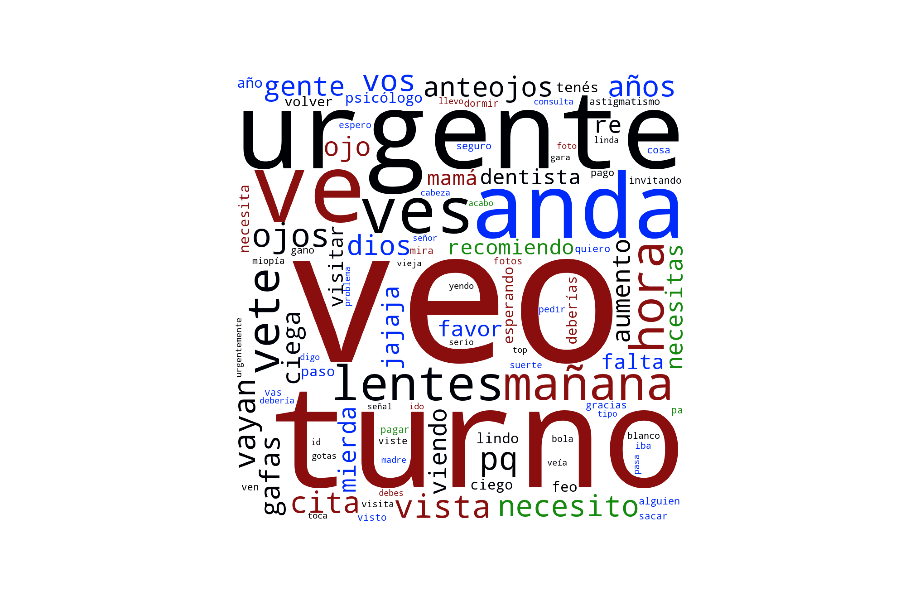
\includegraphics[width=0.7\linewidth]{img/example_structure}
	\caption{Distribución de la palabra oculista. En rojo se muestran los términos concurrentes únicamente con la palabra médico, de verde los términos concurrentes exclusivamente con la palabra abogado y en azul los términos concurrentes con ambas palabras. Gráfico de elaboración propia.}
	\label{fig:example_structure}
\end{figure}


\section{Modelos computacionales con base en la hipótesis distributiva}
\label{sec:sec22}

\cite{otero1975terminologia} menciona que muchos autores definen la conducta lingüística como ``el uso de la palabras'', aunque desde su perspectiva debería limitarse a ser definida como ``el uso de la palabra'' porque se pueden usar palabras sin transmitir un mensaje. ¿Cómo saber que se tiene el uso de la palabra? Desde la perspectiva del PLN esto conoce como Modelado del Lenguaje (ML) y se centra en dos tareas específicas: dada una secuencia de palabras determinar la palabra siguiente y dada una palabra determinar su estructura.

\subsection{N-gramas}
Los modelos que emplearon N-gramas fueron un primer intento de representar las palabras y de resolver la tarea del ML. La idea consiste en calcular la probabilidad de ocurrencia de una secuencia de palabras de longitud $L$. De acuerdo con \cite{brants2007large} dada una secuencia de palabras de longitud $L$, $\left(w_{i_{1}},w_{i_{2}},\ldots,w_{i_{L}}\right)$, su probabilidad de ocurrencia puede calcularse como:
\begin{equation}
	\label{eq:ngrams}
	\footnotesize
	P\left[W_1 =w_{i_{1}},\ldots,W_L =w_{i_{L}}\right] = P\left[W_1=w_{i_{1}}\right] \prod_{j=1}^{L-1}P\left[W_{j+1}=w_{i_{j+1}} |W_1=w_{i_{1}},\ldots,W_j=w_{i_j}\right]
\end{equation}
donde $w_j$ denota la i-ésima palabra del vocabulario, $\{i_j\}_{j=1}^L$ es una colección de índice tales que $i_j = 1,2,\cdots,V$ con $V$ el total de palabras que conforman el vocabulario. De esta forma, las palabras se codifican usando un número natural, sin una preferencia de asignación. De esta forma, la mejor predicción para la palabra siguiente, $w_{L+1}$, dada una secuencia de longitud $L$ es aquella tal que:
\begin{equation}
	\small
	\hat{W}_{L+1} = \arg \max_{1 \leq j \leq V }P\left[W_1 = w_{i_{1}},\ldots,W_L = w_{i_{L}}, W_{L+1}=w_j\right] 
\end{equation}
Note que (\ref{eq:ngrams}) es un conocido resultado de probabilidad\footnote{Se encuentra como ejercicio en el primer capítulo de Introduction to Probability Models de Sheldon Ross.} y que implica genera una cadena con base en las probabilidades condicionadas, es decir, la probabilidad de que la segunda palabra sea cierta palabra depende de la palabra que le antecede, la probabilidad de que la tercera palabra sea una palabra en particular depende de las dos palabras que le anteceden y, así sucesivamente (Fig.~\ref{fig:ngramfull}). 

\begin{figure}[h]
	\centering
		\begin{tikzpicture}[->,>=stealth',auto,semithick,node distance=2cm]
		\tikzstyle{every state}=[draw=black,thick,text=black,scale=1]
		\node[state,fill=black!30!green]    (A)               {$w_1$};
		\node[state,fill=black!30!green]    (B)[right of=A]   {$w_2$};
		\node		    (C)[right of=B]   {$\cdots$};
		\node[state,fill=black!30!green]    (D)[right of=C]   {$w_{L-N+1}$};
		\node		    (E)[right of=D]   {$\cdots$};
		\node[state,fill=white!40!blue]	(F)[right of=E]	  {$w_{L+1}$};
		\path
		(A) edge (B)
		(B) edge (C)
		(C) edge (D)
		(D) edge (E)
		(E) edge (F);
	\end{tikzpicture}
	\caption{Diagrama de una cadena de longitud $L+1$. Donde se muestra que la palabra $w_{L+1}$ depende de todas las palabras anteriores. Gráfico de elaboración propia. }
	\label{fig:ngramfull}
\end{figure}

El cómputo (\ref{eq:ngrams}) se vuelve muy costoso desde el punto de vista de la información requerida $L$ es grande. \cite{norvig209natural} afirma que el cómputo completo para $L=5$ necesitaría aproximadamente 30 GB de información y, es claro que una secuencia de solo 5 palabras es muy limitada. En ese sentido, un supuesto razonable planteado por Brants y su equipo es que la probabilidad de la palabra $L+1$ solo depende de las $N$ palabras anteriores a ésta y no de toda las palabras anteriores (Fig.~\ref{fig:ngram}). De esta forma se tiene la siguiente expresión que se considera el modelo de n-gramas:
\begin{equation}
	\label{eq:ngramsok}
	\scriptsize
	P\left[W_1 = w_{i_{1}},\ldots,W_L = w_{i_{L}}\right] = P\left[W_1=w_{i_{1}}\right] \prod_{j=1}^{L-1}P\left[W_{j+1}=w_{i_{j+1}} |W_{j-N+1}=w_{i_{j-N+1}},\ldots,W_j=w_{i_{j}}\right]
\end{equation}

\begin{figure}[h]
	\centering
	\begin{tikzpicture}[->,>=stealth',auto,semithick,node distance=2cm]
		\tikzstyle{every state}=[draw=black,thick,text=black,scale=1]
		\node[state]    (A)               {$w_1$};
		\node[state]    (B)[right of=A]   {$w_2$};
		\node		    (C)[right of=B]   {$\cdots$};
		\node[state,fill=black!30!green]    (D)[right of=C]   {$w_{L-N+1}$};
		\node		    (E)[right of=D]   {$\cdots$};
		\node[state,fill=white!40!blue]	(F)[right of=E]	  {$w_{L+1}$};
		\path
		(A) edge (B)
		(B) edge (C)
		(C) edge (D)
		(D) edge (E)
		(E) edge (F);
	\end{tikzpicture}
	\caption{Diagrama de una cadena de longitud $L+1$. Donde se muestra que la palabra $w_{L+1}$ depende solo de un número limitado de palabras (en verde). Gráfico de elaboración propia. }
	\label{fig:ngram}
\end{figure}


\subsection{Modelos CBOW y Skip-Gram}

Desde el punto de vista de los modelos basados en n-gramas emplean la distribución de las palabras para cuantificar la incertidumbre sobre la siguiente palabra; pero no permite saltar al nivel semántico. Además de que puede ser cuestionable la reducción para hacer computacionalmente el modelo. \cite{mikolov2013efficient,mikolov2013distributed} proponen que para alcanzar el nivel semántico es necesario emplear otros enfoques. En su trabajo el propone dos modelos: el Modelo de Bolsas de Palabras Continuo (CBOW por sus siglas en inglés) y el modelo Skip-Gram. Ambos modelos basados en redes neuronales secuenciales con tres capas: una capa de entrada, una capa de proyección y una capa de salida (Fig.~\ref{fig:mikolovmodels}).

\begin{figure}[h]
	\centering
	\begin{subfigure}{0.45\linewidth}
		\begin{tikzpicture}[->,>=stealth',auto,semithick,]
			\tikzstyle{every state}=[draw=black,thick,text=black,scale=1]
			\node[state]    (w1)               				  {$\mathbf{W}_L$};
			\node[state]    (w2)[below of=w1, node distance=1.5cm]  				  {$\mathbf{W}_{L-1}$};
			\node[state]    (w3)[below of=w2,node distance=1.7cm]                 {$\mathbf{W}_{L-2}$};
			\node		    (wdot)[below of=w3,node distance=1.1cm]               {$\vdots$};
			\node[state]    (wN)[below of=wdot,node distance=1.5cm]               {$\mathbf{W}_{L-N+1}$};
			\node[state]    (P)[right of=w3,node distance=2.5cm]   				  {$\mathbf{P}$};
			\node[state]    (Y)[right of=P,node distance=2.5cm]   				  {$\mathbf{Y}$};
			\path
			(w1) edge (P)
			(w2) edge (P)
			(w3) edge (P)
			(wN) edge (P)
			(P)  edge (Y);
		\end{tikzpicture}
		\caption{Diagrama de la arquitectura del modelo CBOW. Gráfico de elaboración propia. }
		\label{fig:cbow}
	\end{subfigure}
	\begin{subfigure}{0.45\linewidth}
		\begin{tikzpicture}[->,>=stealth',auto,semithick,]
			\tikzstyle{every state}=[draw=black,thick,text=black,scale=1]
			\node[state]    (w1)               				  {$\mathbf{W}_L$};
			\node[state]    (w2)[below of=w1, node distance=1.5cm]  				  {$\mathbf{W}_{L-1}$};
			\node[state]    (w3)[below of=w2,node distance=1.7cm]                 {$\mathbf{W}_{L-2}$};
			\node		    (wdot)[below of=w3,node distance=1.1cm]               {$\vdots$};
			\node[state]    (wN)[below of=wdot,node distance=1.5cm]               {$\mathbf{W}_{L-N+1}$};
			\node[state]    (P)[left of=w3,node distance=2.5cm]   				  {$\mathbf{P}$};
			\node[state]    (Y)[left of=P,node distance=2.5cm]   				  {$\mathbf{Y}$};
			\path
			(P) edge (wN)
			(P) edge (w3)
			(P) edge (w2)
			(P) edge (w1)
			(Y)  edge (P);
		\end{tikzpicture}
		\caption{Diagrama de la arquitectura del modelo Skip-Gram. }
		\label{fig:skip-gram}
	\end{subfigure}
	\caption{Modelos propuestos por Mikolov para representación y procesamiento de palabras.}
	\label{fig:mikolovmodels}
\end{figure}


El modelo CBOW está enfocado en resolver la misma tarea que los modelos basados en n-gramas: predecir la palabra siguiente dada una sucesión de palabras. Por otro lado, el modelo Skip-Gram permite determinar la distribución de las palabras adyacentes a una palabra dada. En ese sentido, se puede entender que el modelo Skip-Gram es el modelo \textit{inverso} del modelo CBOW. Sin embargo, el enfoque permite:
\begin{enumerate}
	\item Manejar una cantidad más amplía de palabras contexto. Por ejemplo, su trabajo se emplearon 10 palabras contexto.
	\item La proyección permite de alguna manera rescatar la estructura semántica que menciona Harris.
	\item La estructura permite inferir el significado de palabras desconocidas.
\end{enumerate}

El modelo propuesto por Mikolov usualmente se le conoce como \textit{word2vec} y es el enfoque se sigue empleando a la fecha con algunas modificaciones, pero sin perder su esencia. ¿Pero como funciona el modelo? Para ello resulta necesario definir algunos términos. El primer término es la codificación One-Hot, la cual, de acuerdo con \cite{bruce2020practical} se emplean en modelos

\begin{defi}[Codificación One-Hot]
	\label{def:one-hot}
	Dada una variable categórica $X$ con $p$ niveles, una observación de ésta puede codificarse como un vector binario $X'$ de dimensión $p$ donde $1$ índica el nivel observado.
\end{defi}

En los modelos basados en N-gramas cada palabra se puede considerar una variable aleatoria de $V$ niveles, donde $V$ es el número de palabras del vocabulario como ya se mencionó en el apartado anterior. Entonces si la primera palabra de un texto $W_1$ es la i-ésima palabra del vocabulario, $W_1$ puede codificarse como $\bigl[\underbrace{0,\ldots0}_{i-1},1,\underbrace{0,\ldots,0}_{V-i}\bigr]'$.

Luego, según \cite{rong2014word2vec}, el modelo planteado por la Fig.~\ref{fig:cbow} supone que cada palabra se codifica usando One-Hot. En ese sentido, el empleo de $N$ palabras contexto implicaría el empleo de $N\times V$ neuronas de entrada. Sin embargo, un supuesto del modelo de Mikolov consiste en considerar que está proyección es invariante a la posición, es decir, que la información que proporciona una palabra al contexto de otra no depende de su distancia a la palabra sino simplemente si está dentro de una vecindad definida \textit{a priori}\footnote{De ahí el nombre de bolsa de palabras, es como si las palabras se metieran en una bolsa y es esa bolsa la que da el contexto de la palabra.}. En ese sentido, dada una secuencia de $L$ palabras si el contexto de la palabra $L+1$ solo depende de las $N$ palabras anteriores, se tiene que si $\mathbf{P}$ un vector $p$ dimensional es el vector proyección de la capa oculta, entonces:
$$\mathbf{P} = \mathbf{\Omega}'_1 \mathbf{W} $$
donde $\mathbf{W} = \frac{1}{N}\sum_{i=L-N+1}^{L}\mathbf{W}_i$ es un vector de dimensión $V$ y $\mathbf{\Omega}_1$ es la matriz de pesos asociada a la transición entre la capa de entrada y la capa de proyección. Finalmente, lo que se calcula un vector de probabilidades $\mathbf{Y}$ de dimensión $V$ donde cada entrada está asociada a cada una de las palabras del vocabulario. Para ello se emplea la función de activación \textit{softmax}. Así, si $\mathbf{U}$ es el vector proyección resultado de proyectar $\mathbf{P}$, es decir:
$$\mathbf{U} = \mathbf{\Omega}'_2 \mathbf{P} $$
Entonces, la j-ésima entrada de $\mathbf{Y}$ se puede calcular como:
$$y_j = \frac{e^{u_j}}{\sum_{k=1}^{V}e^{u_k}} $$
la anterior expresión corresponde a la función de activación \textit{softmax} y $u_j$ corresponde a la j-ésima entrada el vector $\mathbf{U}$. Similarmente, el modelo planteado por la Fig.~\ref{fig:skip-gram} puede entenderse de manera análoga, solo que en este caso 
$$\mathbf{P} = \mathbf{\Omega}'_1 \mathbf{W} $$
con $\mathbf{W}$ donde es la representación One-Hot de la palabra a proyectar. Note que no se cambia la matriz de pesos del modelo CBOW, \cite{goldberg2014word2vec} mencionan que la matriz de pesos para el modelo Skip-Gram es la misma que para el modelo CBOW. Más aún, debido a la codificación de la palabra a proyectar, la proyección de ésta consiste únicamente de una de las columnas de $\mathbf{\Omega}'$. Por lo tanto, $\mathbf{\Omega}$ posee la información semántica de todo el vocabulario.

\cite{bellegarda2016state} mencionan que $\mathbf{\Omega}$ se le conoce como \textit{embebido de palabras}\footnote{También puede usar el concepto ``encaje de palabras''.}. Además, afirman que es en el espacio vectorial formado por todas las posibles proyecciones donde se encuentra representadas la estructura semántica (Fig.~\ref{fig:word_embedding}) y donde es posible realizar operaciones como $$\mathbf{e}_{\mbox{rey}}-\mathbf{e}_{\mbox{hombre}}+\mathbf{e}_{\mbox{mujer}}=\mathbf{e}_{\mbox{reina}}$$ donde $\mathbf{e}_{w_j}$ es la proyección de la palabra $w_j$. Sin embargo, \cite{goldberg2014word2vec}  menciona que no se conoce la razón por la que el enfoque funciona y que lo único claro es que funciona\footnote{Hasta el 2021 no existe no existe trabajos que den razón del porqué el enfoque de Mikolov refleja lo mencionado en el trabajo de Harris hace ya cerca de siete décadas.}

\begin{figure}[h]
	\centering
	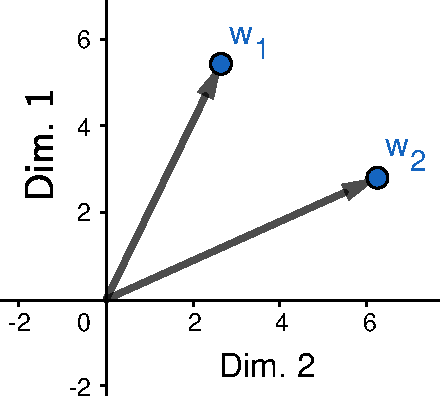
\includegraphics[width=0.7\linewidth]{img/word_embedding}
	\caption{Representación del embebido de palabras bajo $\mathbf{P}$ de dimensión dos. Gráfico de elaboración propia.}
	\label{fig:word_embedding}
\end{figure}

\subsection{Modelo GloVe}

\cite{pennington2014glove} propuso un trabajo en la misma dirección que Mikolov: vectorizar las palabras. Sin embargo, su enfoque parte de una matriz de co-ocurrencias $\mathbf{X}$ donde sus entradas $x_{ij}$ es el número de veces que la j-ésima palabra, $w_j$ del vocabulario aparece en el contexto de la palabra i-ésima, $w_i$. De esta forma, la probabilidad de que la $w_j$ ocurra en el contexto de $w_i$ puede calcularse como sigue:
$$P_{i,j} = \frac{x_{ij}}{x_{i\cdot}}$$
Más aún, Pennington y su equipo hacen las siguientes observaciones:
\begin{itemize}
	\item Das tres palabras $w_{i_1}$, $w_{i_2}$ y $w_{i_3}$. Si $w_{i_3}$ está más relacionada con $w_{i_1}$ que con $w_{i_2}$. Entonces $P_{i_1,i_3} > P_{i_2,i_3}$. Por lo cuál,  se espera que el cociente $P_{i_1,i_3}/P_{i_2,i_3}$ sea grande. Por otro lado, si $w_{i_3}$ está más relacionada con $w_{i_2}$ que con $w_{i_1}$ entonces se esperaría que el cociente $P_{i_1,i_3}/P_{i_2,i_3}$ sea pequeño.
	
	\item Debe existir alguna función $F\left(w_{i_1},w_{i_2},w_{i_3}\right)$ tal que pueda recuperar dichos cocientes. 
	
	\item Esa misma función debe poder capturar el contexto dado por la palabra $w_{i_3}$ y rescatar la diferencia entre las palabras mismas. Por ello, resulta sensato proponer que $$F\left(w_{i_1},w_{i_2},w_{i_3}\right)= F\left(\left(w_{i_1}-w_{i_2}\right)'w_{i_3}\right) = \frac{F\left(w_{i_1}'w_{i_3}\right)}{F\left(w_{i_2}'w_{i_3}\right)}$$
\end{itemize}

Finalmente, el modelo GloVe (Global Vectors) es el par ordenado de matrices $\left(\mathbf{W},\tilde{\mathbf{W}}\right)$ tal que:
\begin{equation}
	\label{eq:glove}
	\ln x_{ij} = \mathbf{w}'_i\tilde{\mathbf{w}}_k + b_i + \tilde{b}_k 
\end{equation}
donde $\mathbf{w}_i$ es la i-ésima columna de $\mathbf{W}$, $\tilde{\mathbf{w}}_k$ la k-ésima columna de $\tilde{\mathbf{W}}$, $b_i$ es una constante de sesgo asociada a la representación de $\mathbf{w}_i$ y, $\tilde{b}_k$ es una constante de sesgo asociada a la representación del contexto de $\tilde{\mathbf{w}}_k$ . Expresión que puede resolverse mediante mínimos cuadrados mediante la siguiente función de error:
\begin{equation}
	\label{eq:glovels}
	E = \sum_{i,j} f\left(x_{ij}\right)\left(\mathbf{w}'_i\tilde{\mathbf{w}}_k + b_i + \tilde{b}_k - \ln x_{ij}\right)^2 
\end{equation}
donde $f$ es una función de penalización dada por:
\begin{equation}
	f(x) = \left\lbrace\begin{array}{ll}
		\left(\frac{x}{100} \right)^{3/4}& \mbox{si } x < 100\\
		1 & \mbox{o.c}
	\end{array} \right.
\end{equation}

\cite{shi2014linking} mencionan que, en la practica, es altamente probable que se tengan varias entradas $x_{ij}=0$ por lo que resulta conveniente sustituir $x_{ij}$ por $x_{ij} +1$. Además de que, las constantes de sesgo no se emplean en la optimización dejando su obtención a un paso posterior empleando algún algoritmo de descomposición de matrices.

\subsection{Sub-palabras}



\section{Pre-procesamiento}
\label{sec:sec23}

\cite{chomsky2004estructuras} menciona que es imposible, solo recolectando locuciones, descubrir todos los patrones existentes en el lenguaje. En ese sentido, lo único que queda es apostar por el volumen. Sin embargo, la cantidad de locuciones revisadas es relativamente pequeña en comparación con la cantidad de locuciones no revisadas que abundan en la red. Por esta razón muchos trabajos han mirado mirado a la web y en particular a las redes sociales, dentro de las cuales resalta Twitter. Sin embargo, de acuerdo con \cite{clark2011text}, la irregularidad de las locuciones hace difícil su uso en aplicaciones de PLN y es por ello que resulta necesario pre-procesar la información.

Las tareas de pre-procesamiento varían en función de las irregularidades de la fuente. En este trabajo, se empleó con la información de la red social Twitter. En ese sentido, \cite{billal2016efficient} mencionan que el pre-procesamiento consiste en tres tareas fundamentales: Normalización, Segmentación y Reconocimiento de Entidades Nombradas (REN).

\subsection{Normalización}
La normalización consiste en darle regularidad a las palabras. En redes sociales es común que para hacer énfasis se repitan algunos de los caracteres que conforman la palabra. Por ejemplo, en lugar de escribir \textit{mucho} se escriba \textit{muuuuucho}. Otro problema con la información obtenida de las redes sociales es la eliminación de las vocales o el cambio de algunos caracteres. Por ejemplo, en lugar de escribir \textit{porque} solo se escribe \textit{pq}. Otro problema clásico son los errores de ortográficos. Por ejemplo, escribir \textit{decisión} en lugar de \textit{decisión}. Sin embargo, de acuerdo con los resultados obtenidos por \cite{hassan2013social}, el problema principal consiste en detectar si en efecto se está ante la presencia de una irregularidad o no. Así, la normalización consiste en una especie de suavizamiento del texto. 

\subsubsection{Problemas por énfasis y expresiones regulares}
Uno puede pensar en la Gramática Generativa de Chomsky en una especie de meta-lenguaje, en el sentido de que, como ya se había mencionado anteriormente, los elementos del lenguaje que propone son oraciones y el alfabeto son los morfemas. Pero note que, a su vez los morfemas con pueden ser elementos de otro lenguaje (una especie de sub-lenguaje) donde, su alfabeto son los caracteres como las letras del abecedario latino.

En la práctica computacional, se sustituye a los morfemas por palabras completas. Así, el lenguaje es una colección de palabras, en lugar de morfemas como proponía Chomsky. De esta forma, en un sentido estricto, el hacer énfasis repitiendo caracteres lleva a que, por ejemplo, palabras como \textit{mucho}, \textit{muuucho} y \textit{muuuuuchoooooo} formen parte del lenguaje. Sin embargo, humanamente todas estas palabras son mapeadas a una única palabra \textit{mucho}. Por lo tanto, el objetivo es poder describir la regularidad presente en el énfasis para luego, hacer el mapeo correspondiente a esa única palabra.

Un de los usos de las expresiones regulares es la realización de tareas como la mencionada en el párrafo anterior. \cite{goyvaerts2012regular} definen una expresión regular como un patrón especifico de texto, es otras palabras, una regularidad en el lenguaje. Formalmente, en teoría de la computación, de acuerdo con \cite{cohen1991introduction} una expresión regular es un subconjunto $A$ de palabras de un lenguaje con un alfabeto $\Sigma$ que puede ser expresadas mediante una serie finita de las siguientes operaciones:

\begin{enumerate}	
	\item \textit{Concatenación.} Dadas dos cadena de caracteres $s_1$ y $s_2$ formadas por una cantidad finita de caracteres del alfabeto $\Sigma$. Se define la concatenación de éstas como $$s_1s_2 = \left\lbrace s_1s_2 \right \rbrace$$
	
	\item \textit{Unión.} Dadas dos cadena de caracteres $s_1$ y $s_2$ formadas por una cantidad finita de caracteres del alfabeto $\Sigma$. Se define la unión de éstas como $$s_1+s_2 = \left\lbrace s_1, s_2 \right \rbrace$$
	
	\item \textit{Estrella de Kleene.} Dada una cadena de caracteres $s$ formada por una cantidad finita de caracteres del alfabeto $\Sigma$. Se define la estrella de Kleene de $s$ como el siguiente conjunto $$s* = \left\lbrace\Lambda, s, ss, sss, \ldots \right \rbrace$$
	
	\item \textit{Estrella positiva de Kleene.} Dada una cadena de caracteres $s$ formada por una cantidad finita de caracteres del alfabeto $\Sigma$. Se define la estrella de Kleene de $s$ como el siguiente conjunto $$s^{+} = \left\lbrace s, ss, sss, \ldots \right \rbrace$$	
\end{enumerate}

De esta manera, es posible describir la regularidad de énfasis de la palabra \textit{mucho} como sigue:
$$mu^+cho^+ = \left\lbrace mucho, muchoo, \ldots, muucho, muuchoo, \ldots, muuucho, muuuchoo, \ldots \right \rbrace$$

Sin embargo, la implementación de expresiones regulares dentro de un lenguaje de programación tiene algunas particularidades extras. En Python, el uso de expresiones regulares se maneja en dos niveles, a nivel de carácter y a nivel de expresión regular.

\paragraph{Nivel de carácter.} En Python, se dice que se trabaja a nivel de carácter cuando se definen lo que se conocen como clases de carácter. Para definir una clase de carácter se emplean corchetes. Así, dados dos caracteres del alfabeto, $c_1$ y $c_2$, se tiene las siguientes equivalencias:
$$[c_1c_2] = \left\lbrace c_1, c_2 \right\rbrace$$
$$[\mbox{\textasciicircum}c_1c_2] = \left\lbrace c_1, c_2 \right\rbrace^{c}$$
Note que las clases de caracteres son subconjuntos de $\Sigma$. Para facilitar la descripción de clases de carácter, Python permite definir de manera corta la clase de minúsculas, mayúsculas y dígitos como: $$[abcd\ldots z] = [a-z]$$ $$[ABCD\ldots Z] = [A-Z]$$ $$[0,1,2\ldots 9] = [0-9]$$ Además, de que existen siete clases de carácter predefinidas y que se muestra en la Tabla~\ref{tb:caracterclassre}.

	\begin{table}[h]
	\centering
	\caption{Expresiones predefinidas en Python. Tabla de elaboración propia con base en lo expuesto en la obra de \cite{lopez2014mastering}. }
	\label{tb:caracterclassre}
		\begin{tabular}{|c|c|}
			\hline
			\textbf{Forma corta} & \textbf{Forma larga}   \\ \hline
			.                    & $[\mbox{\mbox{\textasciicircum}}\mbox{\textbackslash{}}n]$         \\ \hline
			\textbackslash{}d    & $[0-9]$                \\ \hline
			\textbackslash{}D    & $[\mbox{\mbox{\textasciicircum}}0-9]$        \\ \hline
			\textbackslash{}s    & $[\mbox{\textbackslash{}}t\mbox{\textbackslash{}}n\mbox{\textbackslash{}}r\mbox{\textbackslash{}}f\mbox{\textbackslash{}}v]$         \\ \hline
			\textbackslash{}S    & $[\mbox{\mbox{\textasciicircum}}\mbox{\textbackslash{}}t\mbox{\textbackslash{}}b\mbox{\textbackslash{}}r\mbox{\textbackslash{}}f\mbox{\textbackslash{}}v]$ \\ \hline
			\textbackslash{}w    & $[a-zA-Z0-9]$          \\ \hline
			\textbackslash{}W    & $[\mbox{\mbox{\textasciicircum}}a-zA-Z0-9]$  \\ \hline
		\end{tabular}
	\end{table}

Adicional a esto, Python reconoce 4 operaciones generales que puede aplicarse tanto a un carácter como a una clase de carácter:
\begin{itemize}
	\item \textbf{Estrella de Kleene.} La estrella de Kleene se sigue representando por el símbolo asterisco (*).
	
	\item \textbf{Estrella positiva de Kleene.} La estrella positiva de Kleene se sigue representando por el símbolo de suma (+).
	
	\item \textbf{Operación cerradura de pregunta.} En Python símbolo de cerradura de pregunta (?) indica que ese carácter o clase de carácter puede aparecer o no.
	
	\item \textbf{Rango de repeticiones.} En Python puede agregarse al final de un carácter o una clase de carácter $\lbrace\rbrace$ para indicar ciertas repeticiones del carácter o la clase. En ese sentido, $\lbrace n\rbrace$ indica una cantidad fija de repeticiones,  $\lbrace n,\rbrace$ indica una cantidad mínima de repeticiones,  $\lbrace,n\rbrace$ una cantidad máxima de repeticiones y,  $\lbrace n,m\rbrace$ un rango de repeticiones.
\end{itemize}

\paragraph{Nivel de expresión regular.} Para definir una expresión regular en Python esta se escribe entre diagonales como sigue: $$r'\mbox{Expresión regular}'$$
Además para dado que el texto de búsqueda puede ser extenso, Python agrega 6 delimitadores de búsqueda, los cuales se muestran en la Tabla~\ref{tb:redelims}. 
\begin{table}[h]
	\centering
	\caption{Delimitadores de expresiones regulares. Tabla de elaboración propia con base en lo lo expuesto en la obra de \cite{lopez2014mastering}. }
	\label{tb:redelims}
	\begin{tabular}{|c|c|}
		\hline
		\textbf{Notación en Python} & \textbf{Significado}   \\ \hline
		\textasciicircum                    & Inicio de línea         \\ \hline
		\textdollar    & Fin de línea                \\ \hline
		\textbackslash{}b    & Frontera de palabra        \\ \hline
		\textbackslash{}B    & Todo lo que no es frontera de palabra    \\ \hline
		\textbackslash{}A    & Inicio de la entrada \\ \hline
		\textbackslash{}Z    & Fin de entrada         \\ \hline
	\end{tabular}
\end{table}

Para dar claridad sobre el uso de los delimitadores en las expresiones regulares, considere la siguiente entrada:
\begin{quote}
	\textit{Hola Juanito Hola\\
	2Hola Hola Pedrito Hola}
\end{quote}
Así se tiene lo siguiente:
\begin{itemize}
	\item La expresión regular \textit{r'Hola'} hará correspondencia con los todos los \textit{Hola}.
	
	\item La expresión regular \textit{r'\textasciicircum(Hola)'} solo hará correspondencia con el primer \textit{Hola}.
	
	\item La expresión regular \textit{r'(Hola)\textdollar'} solo hará correspondencia con el segundo y último \textit{Hola}.
	
	\item La expresión regular \textit{r'\textbackslash{}bHola'} hará correspondencia con todos los \textit{Hola}, excepto el tercero.
	
	\item La expresión regular \textit{r'\textbackslash{}BHola'} solo hará correspondencia con el tercer \textit{Hola}.
	
	\item La expresión regular \textit{r'\textbackslash{}A(Hola)'} solo hará correspondencia con el primer \textit{Hola}.
	
	\item La expresión regular \textit{r'(Hola)\textbackslash{}Z'} solo hará correspondencia con el último \textit{Hola}.
	
\end{itemize}

 

\paragraph{Generalidades.} Sea cual sea el nivel de descripción, en Python, debido a la notación existen 12 símbolos que no significan el símbolo de forma literal: Diagonal inversa (\textbackslash), intercalación (\textasciicircum), símbolo de dólar (\textdollar), punto (.), barra vertical (\textpipe), cierre de pregunta (?), asterisco (*), símbolo de suma (+), apertura de paréntesis ('('), cerradura de paréntesis (')'), apertura de corchete ([)  y apertura de llave (\{)\footnote{Como nota curiosa en \LaTeX \ la diagonal inversa, la intercalación y el símbolo de dólar también son símbolos prohíbidos}.

\subsubsection{Corrección automática de errores}

\cite{hladek2020survey} mencionan que un algoritmo de corrección de errores consta de tres elementos: diccionario, modelo del error y modelo de contexto, siendo éste último opcional. La idea general es emplear el diccionario para generar candidatos y acomodarlos de acuerdo con el modelo de error y el modelo de contexto.

\paragraph{Modelo del error.} Consiste en evaluar cuál es la viabilidad de cambiar una palabra incorrecta por alguna palabra correcta del diccionario. La viabilidad en este caso se cuantifica por medio de la distancia entre la palabra incorrecta y las palabras del diccionario. Así, dos palabras son igualmente viables como posibles correcciones si su distancia a la palabra incorrecta es la misma. Para ello, \cite{hladek2020survey} mencionan que se emplean principalmente las siguientes funciones de distancia: LD, DLD, LCS las cuales se conocen como métricas o distancias de edición.

\cite{damerau1964technique} menciona una forma de determinar es viable corregir una cadena, $s_1$, por otra cadena, $s_2$, es mediante el empleo de la distancia de Hamming. En este sentido, la corrección es viable si sus longitudes son iguales y la distancia de Hamming entre ambas es a lo sumo 1. \cite{waggener1995pulse} definen la distancia de Hamming para cadenas como sigue:
\begin{defi}[Distancia de Hamming]
	Sean $s_1 = c_{s_1}^1c_{s_1}^2\ldots c_{s_1}^n$ y $s_1 = c_{s_2}^1c_{s_2}^2\ldots c_{s_2}^n$ dos cadenas formadas por $n$ caracteres. Entonces, la distancia de Hamming entre las cadenas está dada por:
	\begin{equation}
		\label{eq:hammingstring}
		d(s_1,s_2) = \sum_{i=1}^{n} I\left(c_{s_1}^i \neq c_{s_2}^i\right)
	\end{equation}
\end{defi}

Por ejemplo, \textit{menestro}\footnote{La siguiente publicación en Twitter \url{https://twitter.com/Justaceo1/status/1379135241898590210} posee el uso \textit{menestro}.} pudiera ser sustituido por \textit{ministro}, \textit{menester} o \textit{maestros}. Luego, empleado (\ref{eq:hammingstring})
$$d(\mbox{menestro},\mbox{ministro}) = 2$$ $$d(\mbox{menestro},\mbox{menester}) = 2$$ $$d(\mbox{menestro},\mbox{maestros}) = 7$$
Por lo que los tres candidatos pueden ordenarse como sigue, $$\mbox{ministro} = \mbox{menester} > \mbox{maestros}$$

Por otro lado, \cite{levenshtein1966binary} identifica tres fuentes de ruido en las cadenas: inserción, eliminación e inversión. La inserción consiste de agregar algún carácter en alguna posición dentro de la cadena original; la eliminación, la operación inversa de la inserción, es la eliminación de algún carácter de la cadena y; la inversión que consiste en permutar una subcadena de la cadena. En ese sentido se define:
\begin{defi}[Distancia LD]
	Sean $s_1$, $s_2$ dos cadenas la distancia LD entre ambas cadenas es el número de inserciones, eliminaciones e inversiones mínimas necesarias para transformar $s_1$ en $s_2$.
\end{defi}
De esta forma, bajo la distancia LD se tiene que:
$$d(\mbox{menestro},\mbox{ministro}) = 4$$ $$d(\mbox{menestro},\mbox{menester}) = 3$$ $$d(\mbox{menestro},\mbox{maestro}) = 3$$ $$d(\mbox{menestro},\mbox{maestros}) = 4$$
Por lo que los cuatros candidatos pueden ordenarse como sigue, $$\mbox{menester} = \mbox{maestro} > \mbox{ministro} = \mbox{maestros}$$
Note que \textit{maestro} ahora puede ser candidato porque en este caso no existe una condición sobre la longitud.

Una tercera alternativa consiste en reconocer una operación adicional a las tres propuesta por Levenshtein: la sustitución. Debido a que, técnicamente, ésta adición es equivalente a mezclar la propuesta de Damerau y Levenshtein, a esta alternativa se le conoce como distancia DLD (Damerau-Levenshtein Distance). Bajo esta alternativa
$$d(\mbox{menestro},\mbox{ministro}) = 2$$ $$d(\mbox{menestro},\mbox{menester}) = 2$$ $$d(\mbox{menestro},\mbox{maestro}) = 2$$ $$d(\mbox{menestro},\mbox{maestros}) = 3$$
Por lo que los cuatros candidatos pueden ordenarse como sigue, $$\mbox{menester} = \mbox{maestro} = \mbox{ministro} > \mbox{maestros}$$

Finalmente, otro criterio para ordenar los candidatos es el criterio de subcadena común más larga con $k$ errores bajo la distancia de Hamming descrito por \cite{flouri2015longest}.

\begin{defi}[Subcadena más larga común]
	Sean $s_1$ y $s_2$ cadenas de longitud $n$ y $m$ con $n \leq m$. Dado un entero $k$ y $\phi(s,i,j)$ subcadena que va del i-ésimo carácter al j-ésimo carácter de una cadena $s$ con $i < j$. La subcadena común más larga con $k$ de $s_1$ y $s_2$, $\phi^{*}$ es tal que:
	
	$$\phi^{*} = \max_{i,j} \phi(s_1,i,j) \quad \mbox{s.a }\quad d(\phi(s_1,i,j),\phi(s_2,i,j))\leq k$$
	donde la distancia es la distancia de Hamming.
\end{defi}

Por ejemplo, si $k = 2$ se tiene que la subcadena más larga con 2 errores de \textit{menestro} respecto \textit{ministro} es \textit{menestro}, respecto \textit{menester} es \textit{menestro}, respecto \textit{maestro} es \textit{men} y, respecto a \textit{maestros} es \textit{men}. Por ende los candidatos pueden ordenarse como:
$$\mbox{menester} = \mbox{ministro} > \mbox{maestro} = \mbox{maestros}$$


\paragraph{Modelo de de contexto.} En el ejemplo de la palabra \textit{menestro}, el contexto:

\begin{quote}
	\textit{mucha vehemencia con las faltas de ortografía de la consejera de Vox en Murcia pero el otro día con la cagada del \textbf{menestro} de Universidades...}
\end{quote} 

deja entrever que la palabra más adecuada es \textit{ministro}. Los modelos de contexto, se encargan de asignar una segunda calificación a los candidatos con base en el contexto, el cual, usualmente está compuesto por las palabras que anteceden al término a corregir.

\cite{hladek2020survey}  menciona que los modelos de contexto empleados para corrección de errores son las GCL, modelos basado en n-gramas, Modelos Ocultos de Markov (MOM), técnicas de aprendizaje máquina como Árboles de Desición, Máquinas de Vectores de Soporte (MVS) o Redes Neuronales (RN). Sin embargo, la herramienta usada varía de lenguaje a lenguaje. En el caso del español, \cite{hladek2020survey} solo identifican cuatro trabajos, de los cuales solo uno de ellos está enfocado al pre-procesamiento de texto proveniente de redes sociales, el trabajo de \cite{melero2016selection}.

Melero y su equipo proponen, para el caso del español, un modelo mixto que consiste en la ponderación de cuatro modelos basados en 3-gramas, el cuál está dado por la siguiente expresión:
\begin{equation}
	\label{eq:melero1}
	\small
	f(s,w^{*}) = \lambda_1f_{TC}(s,w^{*}) + \lambda_2f_{LC}(s,w^{*}) + \lambda_3f_{Lem}(s,w^{*}) + \lambda_4f_{PoS}(s,w^{*})
\end{equation}
donde $s$ es la cadena a corregir\footnote{Se hace la distinción entre palabra y cadena, en el entendido que toda palabra es una cadena pero, no toda cadena es una palabra.} y $w^{*}$ es una palabra candidato, $\lambda_i>0$, $\sum_{i=1}^{4}\lambda_i = 1$ y 
\begin{equation}
	\tiny
	f_{T}(s,w^{*}) = \sum_{i} P\left[w^{*} \in C_{W_n}^i\vert W_{n-1} \in C_{W_{n-1}},W_{n-2} \in C_{W_{n-2}}\right]P\left[W_{n-1} \in C_{W_{n-1}} \vert W_{n-2} \in C_{W_{n-2}}\right]P\left[W_{n-2} \in C_{W_{n-2}}\right]
\end{equation}
donde $T=TC, LC, Lem, PoS$ es el nivel del modelo, $C_{W}$ es la clase de la palabra relativa a $t$. Donde el nivel \textit{TC} se refiere al texto sin transformar, \textit{LC} al texto en minúsculas, \textit{Lem} a la forma lematizada del texto y \textit{PoS} a la forma etiquetada del texto. Por ejemplo, el caso de la cadena \textit{menestro} bajo el modelo de 3-gramas las palabras contexto son \textit{cagada} y \textit{del}, así si para la palabra candidata \textit{ministro}, se tiene: 
$$f_{TC}(s,w^{*}) = f_{TC}(s,w^{*}) = \begin{array}{c}
	P\left[\mbox{ministro} \vert \mbox{del}, \mbox{cagada}\right]	P\left[\mbox{del} \vert \mbox{cagada}\right]P\left[\mbox{cagada}\right]
\end{array}$$
En los primeros dos niveles las clases son las mismas palabras, solo que a nivel \textit{TC} en uno se mantiene la capitalización del texto original y, a nivel \textit{LC} se pasa todo el texto a minúsculas. Por otro lado, para el nivel \textit{Lem} se tiene:
$$f_{Lem}(s,w^{*}) = \begin{array}{c}
	P\left[\mbox{ministro} \vert \mbox{del}, \mbox{cagar}\right]	P\left[\mbox{del} \vert \mbox{cagar}\right]P\left[\mbox{cagar}\right]
\end{array}$$
Mientras que a nivel \textit{PoS} se tiene:
$$\small f_{PoS}(s,w^{*}) = \begin{array}{c}
	P\left[\mbox{sustantivo} \vert \mbox{determinante}, \mbox{sustantivo}\right]	P\left[\mbox{determinante} \vert \mbox{sustantivo}\right]P\left[\mbox{sustantivo}\right]
\end{array}$$

Sin embargo, Melero y su equipo estiman que $\lambda_4 = 0$, $\lambda_3 = 0.0962$ y $\lambda_1=\lambda_2 = 0.4519$. Con lo que (\ref{eq:melero1}) puede reducirse a:
\begin{equation}
	\label{eq:melero2}
	f(s,w^{*}) \approx 0.4519f_{TC}(s,w^{*}) + 0.4519f_{LC}(s,w^{*}) 
\end{equation}

\subsection{Segmentación}

En Twitter parte de la información está contenida en lo que se denomina \textit{hashtag}, los cuales organizan la información por temas o eventos \citep{small2011hashtag}. Por ejemplo, el tweet:

\begin{quotation}
	\#Anticonvocatoria donde nada \#CambiaElJuego todo lo que escucho es \#AMLOLujoDePresidente efímero y devaluado igual \#Letrinus y todos los demás.\\ \begin{flushright}
		\textit{-@causa\_nuestra}\footnote{El tweet puede ser consultado en \url{https://twitter.com/causa_nuestra/status/1377178856193359874}}
	\end{flushright}
\end{quotation}
contiene cuatro \textit{hashtags} de los cuáles dos tiene información que debe ser segmentada: \textit{Cambia el juego} y \textit{AMLO lujo de presidente}. En ese sentido, el algoritmo más usado de segmentación es el algoritmo basado en uni-gramas y 2-gramas propuesto por \cite{norvig209natural}. En su trabajo Norvig propone dada una cadena $s_0$ se puede segmentar como $s_0 = w_1s_1$, donde a su vez se puede segmentar $s_1 = w_2s_2$ y, así sucesivamente, donde $s_{i+1}$ es la cadena sobrante al quitar $w_{i+1}$ de la cadena $s_{i}$ y
\begin{equation}
	\label{eq:norvig}
	w_{i+1} = \arg\max_{w^{*}} P\left[w_{i+1} \vert w_{i}\right]P\left[w_{i}\right]P[s_{i+1}]
\end{equation}
donde $P[s_{i+1}]$ funciona como un ponderador y las probabilidades se calculan usando la distribución de frecuencias del \textit{corpus}. Sin embargo, como en la mayoría de los casos las cadenas $s_i$ no son palabras, entonces Norvig propone un modelo probabilístico para palabras desconocidas dada por la siguiente expresión:
\begin{equation}
	\label{eq:norvigunknown}
	P[s] = \frac{10}{\vert s \vert 10^{\vert s \vert}}
\end{equation}
Sin embargo, Norvig comenta que la expresión anterior no tiene ningún sustento teórico y se debe a un ajuste empírico. En ese sentido, \cite{cano2019segmentacion} encontró que, para el caso del español, una mejor alternativa es el uso de un modelo de probabilidad Weibuill discreta de parámetros $\alpha = 7.5291$ y $\beta = 2.2066$ donde la variable aleatoria sigue estando en términos de la longitud de la cadena.

\subsection{Reconocimiento de Entidades Nombradas}

El REN consiste en identificar sustantivos propios, algunas abreviaturas como el tipo de moneda o fechas en el texto. Los nombre de los países, ciudades y nombres propios son ejemplos de entidades nombradas. Usualmente, éstas están compuestas por una sola \textit{palabra}, como \textit{Mexicali}, \textit{México} o \textit{Juan}. Sin embargo, no todas las entidades nombradas son de una palabra. Por ejemplo:

\begin{quotation}
	Cierto. Algo tuve que ver representando a un \textbf{Instituto Universitario Tecnológico}.\\ \begin{flushright}
		\textit{-@castellimika}\footnote{El tweet puede ser consultado en \url{https://twitter.com/castellimika/status/1379226926028587009}}
	\end{flushright}
\end{quotation}
En este sentido \textit{Instituto Universitario Tecnológico} es una entidad nombrada. Dentro del texto formal, las entidades nombradas tienen la característica de estar capitalizadas; pero dentro del texto informal esto no siempre ocurre. Por ejemplo, en el siguiente tweet además de otros errores se puede apreciar que la entidad nombrada \textit{Mexicali} no está capitalizada.

\begin{quotation}
	Otro gran lunes como cada semana \#LaMesaRenonaEnVivo saludos @franco\_esca @elchristianmeza @lamolechida desde \textbf{mexicali} por otra gran noche de risas \#soytoronto y tambien saludos para el rubiiiiiiiiiii me encanta que le cagues la vida al @elchristianmeza\\ \begin{flushright}
		\textit{-@bambino03garcia
		}\footnote{El tweet puede ser consultado en \url{https://twitter.com/bambino03garcia/status/1379275928233107458}}
	\end{flushright}
\end{quotation}

\cite{nouvel2016named} reconocen que existen cinco enfoques para el REN, cuatro supervizados: Naïve Bayes, MOM, Redes Neuronales y los Campos Aleatorios Condicionales (CAC) y uno no supervizado basado en semántica. Siendo los CAC de Cadena Lineal el enfoque con mejores resultados en la tarea.

Debido a la relación que tienen los CAC con los MOM, se empezarán a describir los MOM primero. \cite{ross2014introduction} define estos como sigue:

\begin{defi}[Modelo de Markov Oculto]
	Sea $\left\lbrace X_i, i=1,2,\ldots\right\rbrace$ una cadena de Markov con probabilidades de transición $P_{ij}$ y probabilidades de estado inicial $p_i$. Suponga también que, existe un conjunto finito de señales $\mathcal{S}$ que se emite cada que la cadena de Markov entra a un estado. Además, considere que cuando la cadena de Markov entra a un estado $j$ entonces, independientemente del estado previo de la cadena y la señales previas, la probabilidad de que la señal emitada sea $s$ solo depende del estado actual $j$, es decir, $p(s|j)$ de esta forma si $S_i$ denota la i-ésima señal emitida se tiene que:
	$$p(s|j) = P\left[S_n \vert X_1,S_1,X_2,S_2\ldots,X_{n-1},S_{n-1},X_{n}=j\right]$$
	En ese sentido, note que las señales $S_1,S_2\ldots$ serán una secuencia de estados observable mientras la cadena $X_1,X_2\ldots$ no lo será, siendo está una cadena de Markov oculta, y al modelo de probabilidades de transición se le conoce como Modelo de Markov Oculto (MOM).
\end{defi}

Desde el punto de vista del NER, las señales son la palabras, $W$ y, los estados de la cadena no observable las etiquetas asociadas al NER, $S$ (Fig.~\ref{fig:hmms}). Note que, adecuando la definición al contexto del NER, se tiene que:
$$p(s|j) = P\left[W_{L+1} = w_j | S_1,W_1,S_2,W_2\ldots,S_{L},W_{L},S_{L}=s_j\right]$$ Aunque, desde el punto de vista de la aplicación se está interesado en calcular para $k\leq L$ la probabilidad de que la k-ésima entidad sea de la clase $s_j$ usando la información dada por las señales, es decir:

\begin{equation}
	\label{eq:ner1}
	P\left[S_{k} = s_j | S_1=s_{i_1},S_2=s_{i_2},\ldots,S_L=s_{i_L}\right]
\end{equation}

\cite{nouvel2016named} menciona que, a menudo en el contexto de la NER, se acostumbra calcular de probabilidad de que una sucesión de entidades tenga ciertas etiquetas, en lugar de lo planteado en (\ref{eq:ner1}. De esta forma, si se conocen las etiquetas de las primeras $k$ entidades, la idea es encontrar las clases o etiquetas $s_{j_1},s_{j_2},\ldots,s_{j_L}$ tales que se maximice 
\begin{equation}
	\label{eq:hmmsolve}
	P\left[S_{1} = s_{j_1}, \ldots, S_{L} = s_{j_L} | W_1=w_{i_1},\ldots,W_L=w_{i_L}\right]
\end{equation}
dado que, como ya se mencionó se conocen los primeros $k$ estados de la cadena no observable.

\begin{figure}[h]
	\centering
	\begin{subfigure}{0.7\linewidth}
		\centering
		\begin{tikzpicture}[->,>=stealth',auto,semithick,node distance=2cm]
			\tikzstyle{every state}=[draw=black,thick,text=black,scale=1]
			\node[state,fill=black!30!green]    (A)               {$X_1$};
			\node[state,fill=black!30!green]    (B)[right of=A]   {$X_2$};
			\node		    (C)[right of=B]   {$\cdots$};
			\node[state,fill=black!30!green]	(D)[right of=C]	  {$X_{n}$};
			\node		    (E)[right of=D]   {$\cdots$};
			\node[state,fill=white!40!blue]    (Ab)[below of=A]   {$S_1$};
			\node[state,fill=white!40!blue]    (Bb)[right of=Ab]   {$S_2$};
			\node		    (Cb)[right of=Bb]   {$\cdots$};
			\node[state,fill=white!40!blue]	(Db)[right of=Cb]	  {$S_{n}$};
			\node		    (Eb)[right of=Db]   {$\cdots$};
			\path
			(A) edge (B)
			(B) edge (C)
			(C) edge (D)
			(D) edge (E)
			(A) edge (Ab)
			(B) edge (Bb)
			(D) edge (Db);
		\end{tikzpicture}
		\caption{Diagrama de un Modelo de Markov Oculto. Gráfico de elaboración propia. }
		\label{fig:hmm}
	\end{subfigure}
	\begin{subfigure}{\linewidth}
		\centering
		\begin{tikzpicture}[->,>=stealth',auto,semithick,node distance=2cm]
			\tikzstyle{every state}=[draw=black,thick,text=black,scale=1]
			\node[state,fill=black!30!green]    (A)               {O};
			\node[state,fill=black!30!green]    (Bc)[right of=A]   {O};
			\node[state,fill=black!30!green]    (B)[right of=Bc]   {Día};
			\node		    (C)[right of=B]   {$\cdots$};
			\node[state,fill=black!30!green]	(Dc)[right of=C]	  {O};
			\node[state,fill=black!30!green]	(D)[right of=Dc]	  {?};
			\node		    (E)[right of=D]   {$\cdots$};
			\node[state,fill=white!40!blue]    (Ab)[below of=A]   {Otro};
			\node[state,fill=white!40!blue]    (Bcb)[right of=Ab]   {gran};
			\node[state,fill=white!40!blue]    (Bb)[right of=Bcb]   {lunes};
			\node		    (Cb)[right of=Bb]   {$\cdots$};
			\node[state,fill=white!40!blue]	(Db)[right of=Cb]	  {desde};
			\node[state,fill=white!40!blue]	(Eb)[right of=Db]	  {mexicali};
			\node		    (Ec)[right of=Eb]   {$\cdots$};
			\path
			(A) edge (Bc)
			(Bc) edge (B)
			(B) edge (C)
			(C) edge (Dc)
			(Dc) edge (D)
			(D) edge (E)
			(A) edge (Ab)
			(Bc) edge (Bcb)
			(B) edge (Bb)
			(Dc) edge (Db)
			(D) edge (Eb);
		\end{tikzpicture}
		\caption{Diagrama de un Modelo de Markov Oculto en el contexto del NER aplicado al segundo tweet de ejemplo en este apartado. En este caso, la etiqueta 'O' significa 'Otro' para denotar que no es una entidad nombrada. Gráfico de elaboración propia. }
		\label{fig:hmmner}
	\end{subfigure}
	\caption{Diagrama de Modelo Oculto de Markov, en verde se muestra la cadena de Markov oculta y en azul las señales observables.}
	\label{fig:hmms}
\end{figure}

La expresión planteada por (\ref{eq:hmmsolve}) usualmente se resuelve recursivamente empleando el algoritmo de Viterbi. En lo que respecta a los CAC de Cadena Lineal, estos son una generalización de los MOM. Para ello, note que la expresión (\ref{eq:hmmsolve}) por definición de probabilidad condicionada es equivalente a:
\begin{equation}
	\label{eq:hmmsolveequiv1}
	\scriptsize
	P\left[S_{1} = s_{j_1}, \ldots, S_{L} = s_{j_L} | W_1=w_{i_1},\ldots,W_L=w_{i_L}\right] = \frac{	P\left[S_{1} = s_{j_1}, \ldots, S_{L} = s_{j_L}, W_1=w_{i_1},\ldots,W_L=w_{i_L}\right]}{	P\left[W_1=w_{i_1},\ldots,W_L=w_{i_L}\right]}
\end{equation}
La cual por la propiedad markoviana, la independencia de las señales puede reescribirse como y aplicando marginalización:
\begin{equation}
	\label{eq:hmmsolveequiv2}
	\tiny
		P\left[S_{1} = s_{j_1}, \ldots, S_{L} = s_{j_L} | W_1=w_{i_1},\ldots,W_L=w_{i_L}\right] = \frac{\prod_{h=1}^{n}P\left[S_{h}=s_{j_h}\vert S_{h-1}=s_{j_{h-1}}\right]P\left[W_{h}=w_{i_h}\vert S_{h}=s_{j_h}\right]}{\sum_{\mathbf{s}}\prod_{h=1}^{n}P\left[S_{h}=s_{j_h}\vert S_{h-1}=s_{j_{h-1}}\right]P\left[W_{h}=w_{i_h}\vert S_{h}=s_{j_h}\right]}
\end{equation}
Definiendo $\theta_{j_i,j_{i-1}} = \ln P\left[X_{i}=j_i\vert X_{i-1}=j_{i-1}\right]$ y $\mu_{s_i,j_i} = \ln P\left[S_{i}=s_i\vert X_{i}=j_i\right]$ la expresión anterior puede volver a escribir como:
\begin{equation}
	\label{eq:hmmsolveequiv3}
	\small
	P\left[X_{1} = j_1, \ldots, X_{n} = j_n | S_1=s_1,\ldots,S_n=s_n\right] = \frac{\prod_{i=1}^{n}\exp \left\lbrace \theta_{j_i,j_{i-1}} + \mu_{s_i,j_i} \right\rbrace}{\sum_{\mathbf{s}}\prod_{i=1}^{n}\exp \left\lbrace \theta_{j_i,j_{i-1}} + \mu_{s_i,j_i} \right\rbrace}
\end{equation}
Finalmente, esta última expresión puede escribirse como:
\begin{equation}
	\label{eq:hmmsolveequiv4}
	\scriptsize
	\frac{\prod_{i=1}^{n}\exp \left\lbrace \sum_{j_i,j_{i-1} \in J}\theta_{j_i,j_{i-1}}I\left(X_{i}=j_i\right)I\left(X_{i-1}=j_{i-1}\right) + \sum_{j_i \in J}\sum_{s_i \in S}\mu_{s_i,j_i}I\left(X_{i}=j_i\right)I\left(S_{i}=s_i\right) \right\rbrace}{\sum_{\mathbf{s}}\prod_{i=1}^{n}\exp \left\lbrace \sum_{j_i,j_{i-1} \in J}\theta_{j_i,j_{i-1}}I\left(X_{i}=j_i\right)I\left(X_{i-1}=j_{i-1}\right) + \sum_{j_i \in J}\sum_{s_i \in S}\mu_{s_i,j_i}I\left(X_{i}=j_i\right)I\left(S_{i}=s_i\right) \right\rbrace}
\end{equation}

Por otro lado, \cite{sutton2019introduction} define un CAC de Cadena Lineal como sigue:

\begin{defi}[Campo Aleatorio Condicional de Cadena Lineal]
	\label{def:caccl}
	Sean $\mathbf{S}$ y $\mathbf{X}$ vectores aleatorios, $\mathbf{\theta} \in \mathbb{R}^K$ un vector de parámetros y, $\mathcal{F} = \left\lbrace f_{k}(x,x',\mathbf{s}_i)\right\rbrace_{k=1}^K$ un conjunto de funciones reales, que se llamarán funciones de características. Entonces un Campo Aleatorio Condicional de Cadena Lineal es la condicionada de $\mathbf{X}\vert \mathbf{S}$ tal que esta puede escribirse como:
	\begin{equation}
		P[\mathbf{X}=\mathbf{x}| \mathbf{S}=\mathbf{s}] = \frac{1}{Z(\mathbf{x})}\prod_{t=1}^{T}\exp \left\lbrace \sum_{k=1}^{K}\theta_k f_k\left(x_t,x_{t-1},\mathbf{s}_t\right)\right\rbrace
	\end{equation}
	con
	\begin{equation}
		Z\left(\mathbf{x}\right) = \sum_{\mathbf{s}}\prod_{t=1}^{T}\exp \left\lbrace \sum_{k=1}^{K}\theta_k f_k\left(x_t,x_{t-1},\mathbf{s}_t\right)\right\rbrace
	\end{equation}
\end{defi}

Note que usando la Def.~\ref{def:caccl} con $K$ es el total de índices que recorren las sumas planteadas por (\ref{eq:hmmsolveequiv4}), las funciones indicadoras de esa misma función como las funciones de características y $\theta_{j_i,j_{i-1}}$ y $\mu_{s_i,j_i}$ como parámetros entonces se tiene que el MOM cumple con la definición de un CAC de Cadena Lineal. Pero, note que la definición permite el uso de funciones de características más elaboradas.

\textbf{Falta diagrama}

\section{Optimización}

La estimación de los modelos y tareas de pre-procesamiento mencionadas en apartados anteriores implican una tarea de optimización. En este apartado describimos los métodos de optimización que fueron empleados en este trabajo, aunque la solución del problema de optimización no está de ninguna manera limitado al uso único de las tareas mencionadas.

\subsection{Estimación de los modelos CBOW y Skip-Gram}

\cite{mikolov2013efficient} describe que la tarea de estimación usando directamente el algoritmo propagación hacia atrás puede resultar muy costoso computacionalmente. Para ello, propone reducir la carga operacional mediante la aplicación de uno de los siguientes dos enfoques: muestreo negativo y optimización jerárquica.

\paragraph{Muestreo negativo.} De acuerdo con \cite{rong2014word2vec} la función de pérdida del modelo CBOW está dada por la siguiente expresión:
\begin{equation}
	\label{eq:losscbow}
	E = - \mathbf{W}'_{L+1}\mathbf{P} + \ln \left(\sum_{i=1}^{V} \exp\left\lbrace \mathbf{W}'_{i}\mathbf{P}\right\rbrace\right)
\end{equation}

De acuerdo con \cite{goldberg2014word2vec}, el muestreo negativo consiste en cambiar la función de pérdida planteada por (\ref{eq:losscbow}) por la siguiente expresión:
\begin{equation}
	\label{eq:losscbow2}
	E = - \ln \sigma\left(\mathbf{W}'_{L+1}\mathbf{P}\right) - \sum_{i \in I_{neg}} \ln \sigma\left(\mathbf{W}'_{i}\mathbf{P}\right)
\end{equation}
donde $I_{neg}$ es un conjunto de índices tal que $I_{neg} \subset \left\lbrace1,2,\ldots,V\right\rbrace$. De esta forma se reducen las operaciones necesarias para aplicar el algoritmo de propagación hacia atrás. Aunque es necesario aclarar que las funciones de optimización no son equivalente, pero de acuerdo con \cite{goldberg2014word2vec} las representaciones obtenidas son similares a las que se obtendrían usando (\ref{eq:losscbow}).

\paragraph{Optimización jerárquica.} El objetivo del modelo CBOW en poder calcular
\begin{equation}
	y_j = \frac{e^{u_j}}{\sum_{k=1}^{V}e^{u_k}} 
\end{equation}
es decir, la probabilidad de que la palabra siguiente con base en el contexto dado. Matemáticamente,
\begin{equation}
	\label{eq:optijerar1}
	P\left[W_{L+1} = w_j \vert W_{L}=w_{i_{L}},\ldots,W_{L-N+1}=w_{i_{L-N+1}}\right]
\end{equation} 
En ese sentido, el método de optimización jerárquica tiene sustento en el trabajo publicado por \cite{morin2005hierarchical} que afirma que si el vocabulario puede dividirse en una colección de subconjuntos disjuntos, tal que existe una función $c$ que a cada palabra le asigna con uno de esos subconjuntos $c\left(w_j\right)$ entonces resulta más eficiente calcular (\ref{eq:optijerar1}) por medio de la siguiente igualdad:
\begin{equation}
	\tiny
	 P\left[W_{L+1} = w_j | C = c(w_j), W_{L}=w_{i_{L}},\ldots,W_{L-N+1}=w_{i_{L-N+1}}\right]P\left[C=c(w_j)|W_{L}=w_{i_{L}},\ldots,W_{L-N+1}=w_{i_{L-N+1}}\right]
\end{equation}
De esta forma, un problema donde la etiqueta tiene $p$ niveles se transforma en $p$ problemas de etiquetas binarias, el cuál es más sencillo de resolver.

\paragraph{Algoritmo de propagación hacia atrás.} El objetivo del algoritmo de propagación hacia atrás (BP por sus siglas en inglés) consiste en minimizar la función de pérdida de una red neuronal por medio del gradiente de la función de error \citep{rojas1996backpropagation}. En otras, palabras la idea cuantificar las variaciones del error causas por las variaciones en las entradas.  Sin embargo, cuando la arquitectura de una red neuronal posee, al menos, una capa de oculta, no se puede cuantificar directamente. 

Por ejemplo, en el caso de la función de pérdida planteada por (\ref{eq:losscbow2}) en una primera etapa, por medio del método del gradiente se tiene que:
\begin{equation}
	W_{L+1}^{'\mbox{nuevo}} = W_{L+1}^{'\mbox{viejo}} - \eta \frac{\partial E}{\partial \mathbf{W}'_{L+1}\mathbf{P}} \cdot \frac{\partial \mathbf{W}'_{L+1}\mathbf{P}}{\partial \mathbf{W}'_{L+1}}
\end{equation}

Sin embargo, la expresión solo permite actualizar segunda matriz de pesos, para actualizar la primera y dado que la proyección tiene una función de activación lineal, basta ver como varian las proyecciones en función de las entradas. Así, nuevamente por el método del gradiente

\begin{equation}
	W_{L+1}^{\mbox{nuevo}} = W_{L+1}^{\mbox{viejo}} - \frac{1}{N}\eta\frac{\partial E}{\partial \mathbf{W}'_{L+1}\mathbf{P}} \cdot \frac{\partial \mathbf{W}'_{L+1}\mathbf{P}}{\partial \mathbf{P}}
\end{equation}


\subsection{Algoritmo de Viterbi}

\subsection{Algoritmos meta-heurísticos: Evolución diferencial}

\section{Sobre la similitud semántica}
\label{sec:sec25}

Los modelos CBOW, Skip-Gram y GloVe como se mencionó en la sección~\ref{sec:sec21} tienen el beneficio de recuperar la estructura semántica de las palabras. Mediante su aplicación cada palabra es representada como un punto en el espacio y entonces dos palabras están relacionadas si la distancia entre sus representaciones es pequeña. 

\cite{bellegarda2016state} mencionan que, lo más común para determinar la similitud semántica entre dos proyecciones $\mathbf{e}_{w_j}$ y $\mathbf{e}_{w_k}$ es mediante cualquiera de las siguientes dos funciones de distancia:
\begin{align*}
	d_1\left(\mathbf{e}_{w_j},\mathbf{e}_{w_k}\right) = \sqrt{\sum_{h=1}^p \left(e_{w_j}^h -e_{w_k}^h\right)^2} & \quad \mbox{Distancia Euclideana}\\
	d_2\left(\mathbf{e}_{w_j},\mathbf{e}_{w_k}\right) = \frac{\mathbf{e}_{w_j}\cdot \mathbf{e}_{w_k}}{\left\lVert\mathbf{e}_{w_j}\right\rVert\left\lVert\mathbf{e}_{w_k}\right\rVert} & \quad \mbox{Ángulo entre vectores}
\end{align*}
donde $e_{w_j}^h$ es la h-ésima entrada de la proyección.

En muchas áreas, el concepto de distancia está relacionado con el concepto de similitud. En ese sentido, la propuesta de este trabajo como se mencionó en el \textbf{sección de hipótesis} es observar el comportamiento del embebido bajo otras funciones de distancia, en particular, bajo la distancia de Hausdoff. Entonces, ¿cuál es la distancia de Haussdoff? \cite{munkres2000topolgy} define la distancia de Hausdoff entre dos conjuntos no vacíos $A$ y $B$ de un espacio métrico como:
\begin{equation}
	\label{eq:hausdoff_original}
	d_H\left(A,B\right) = \max \left\lbrace \sup_{a\in A} d(a,B),\sup_{b\in B}d(A,b)\right\rbrace
\end{equation}
donde $d(a,B) = \inf_{b\in B}d(a,b)$. Así, considere que cada una de las  proyecciones $\mathbf{e}_{w_j}$ y $\mathbf{e}_{w_k}$ es un conjunto de $p$ características $e_{w}^h$. Entonces, (\ref{eq:hausdoff_original}) aplicado al contexto de se puede ver expresare como:
\begin{equation}
	\label{eq:hausdoff_words}
	d_H\left(\mathbf{e}_{w_j},\mathbf{e}_{w_k}\right) = \max \left\lbrace \sup_{1\leq h\leq p} d(e_{w_j}^h,\mathbf{e}_{w_k}),\sup_{1 \leq h' \leq p}d(\mathbf{e}_{w_j},e_{w_k}^{h'})\right\rbrace
\end{equation}
donde $d(e_{w_j}^h,\mathbf{e}_{w_k}) = \inf_{i \leq h \leq p}\lvert e_{w_j}^h-e_{w_k}^h\rvert$

\subsection{Silabeo}


\subsection{Sobre aplicaciones terminales}


\section{Teoría lingüística adicional}



\chapter{Metodología}
\label{ch:chap3}
% \epigraph{\textit{``Una terrible verdad es mejor que una \'util mentira"}}{--- \textup{Thoman Mann}, La monta\~na m\'agica}

\section{Obtención de locuciones}

En la sección~\ref{sec:sec21} se mencionó que la clave para poder aproximar la estructura lingüística era por medio de una colección de locuciones. Mientras que, en la sección~\ref{sec:sec23} se mencionó que en muchas ocasiones se recurre a las redes sociales para obtener dicha colección. La búsqueda y obtención de locuciones en este trabajo puede resumirse en dos pasos:

\begin{enumerate}
	\item Determinación de las locuciones a buscar
	\item Búsqueda de las locuciones especificadas.
\end{enumerate}

\paragraph{Determinación de las locuciones a buscar.} Al recurrir a las redes sociales, lo primero que debe hacerse es determinar lo que hay que buscar. Para ello, en este trabajo se emplearon los datos proporcionados por \cite{crearae}\footnote{En marzo de 2021 la RAE publica una versión anotada del CREA. Sin embargo contiene una revisión de documentos menos reciente pues solo analiza documentos publicados entre el año 1975 y el año 2000.} que, de cuerdo con Real Academia Española (RAE) consta de una amplía variedad de textos de habla hispana desde 1975 hasta 2004 y una lista de más de 700,000 locuciones del español.

\begin{table}[h]
	\caption{Lista de las 10 palabras más frecuentes en el español de acuerdo con el CREA.}
	\label{tb:creafreq}
	\centering
	\begin{tabular}{|c|c|}
		\hline
		\textbf{Palabra} & \textbf{Frecuencia} \\ \hline
		de               & 9,999,518           \\ \hline
		la               & 6,277,560           \\ \hline
		que              & 4,681,839           \\ \hline
		el               & 4,569,652           \\ \hline
		en               & 4,234,281           \\ \hline
		y                & 4,180,279           \\ \hline
		a                & 3,260,939           \\ \hline
		los              & 2,618,657           \\ \hline
		se               & 2,022,514           \\ \hline
		del              & 1,857,225           \\ \hline
	\end{tabular}
\end{table}

El CREA proporciona la lista de locuciones y la frecuencia de aparición dentro de un conjunto de 140,000 documentos analizados (Tabla~\ref{tb:creafreq}). Sin embargo, en la práctica la inclusión de algunas palabras puede ocasionar efectos no deseados en la estimación de los modelos empleados en el PLN. Para ello, desde el nacimiento del PLN se ha hecho empleo de un conjunto llamado \textit{stop-words} o diccionario negativo el consta de una lista de términos que se excluyen en la estimación del modelo para mejorar los resultados obtenidos en tareas de PLN \citep{fox1989stop}. En el caso del español, el trabajo publicado por \cite{stopwords_es} ha recibido mucha aceptación, por lo que su diccionario negativo de 990 palabras fue el que se empleó para filtrar algunas de las palabras de la lista original del CREA (Tabla~\ref{tb:creafreq_filtered}).

\begin{table}[h]
	\caption{Lista de las 10 palabras más frecuentes en el español de acuerdo con el CREA excluyendo las palabras del diccionario negativo.}
	\label{tb:creafreq_filtered}
	\centering
	\begin{tabular}{|c|c|}
		\hline
		\textbf{Palabra} & \textbf{Frecuencia} \\ \hline
		años             & 203,027             \\ \hline
		vida             & 123,491             \\ \hline
		gobierno         & 113,011             \\ \hline
		país             & 104,568             \\ \hline
		mundo            & 101,745             \\ \hline
		año              & 100,790             \\ \hline
		forma            & 97,165              \\ \hline
		caso             & 96,979              \\ \hline
		millones         & 81,999              \\ \hline
		españa           & 80,195              \\ \hline
	\end{tabular}
\end{table}

\paragraph{Búsqueda de las locuciones especificadas.} La búsqueda, al momento de escribir esta tesis, es tan sencilla como buscar en algo en Google. Sin embargo, para poder llegar a estas alturas fue necesario hacer lo siguiente:
\begin{enumerate}
	\item Configuración del acceso remoto a la red social.
	\item Procesamiento de la información obtenida, que consiste en la descarga, lectura de la información y almacenamiento en legible de la información obtenida.
\end{enumerate}

La mayoría de las redes sociales ofrece un acceso remoto a su red social con el fin de apoyar a sus clientes que usualmente son compañías que buscan alguna interacción con los usuarios del la misma. Para ello, \cite{twitterdev} ofrece una opción para desarrolladores abierta a cualquier persona u organización enfocada a cuatro tareas principales: Oir y analizar, lo cual consiste en proporcionar acceso a las publicaciones públicas de los usuarios de la red social; Publicidad, lo cual consiste en proveer herramientas para manejar campañas publicitarias dentro de la red social; Publicación, lo cuál consiste en ofrecer herramientas el manejo de imagen y publicaciones de instituciones dentro de la red social y; Captación, que en un conjunto de herramientas que permite dirigir usuarios hacia ciertos contenidos\footnote{La cuenta que se empleó en este trabajo fue creada en 2017, época en la cual no hacia falta más que crear una cuenta en la red social y activar la opción de desarrollador. Sin embargo, después del escándalo ocasionado por Cambridge Analytica en 2018, la creación de una cuenta de desarrollador debe tramitarse y esperar autorización.}.

Para el acceso remoto de cualquier servicio en línea, los prestadores del servicio permiten a los desarrolladores interactuar con sus servicios por medio de una API (Application Programming Interface), la cuál sirve como intermediario entre el lenguaje que emplea el desarrollador y los sistemas del provedor. En este trabajo se empleó la biblioteca \textit{tweepy} v3.8 creada por \cite{tweepy} que sirve como un intermediario de fácil uso entre la API de Twitter y Python y posteriormente se empleeo el script \textit{get\_expressions.py} disponible en mi página de GitHub personal (ver \nameref{ch:prefacio}.)  para obtener 100 publicaciones para cada una de las locuciones contenidas en la lista del CREA con una frecuencia superior a 30 y que no estuvieran contenidas en el diccionario negativo. En total 100,337 locuciones fueron buscadas y se obtuvieron en la mayoría de los casos 100 publicaciones donde aparecían éstas. Lo que dio un total de de 10,033,700 de publicaciones obtenidas y procesadas, donde cada publicación cuenta con un promedio de 10 palabras, por lo que en total se formó una colección de aproximadamente 100,337,000 elementos\footnote{La información recabada representa aproximadamente tan solo 1.8 GB de información. Sin embargo, si el lector, desea aventurarse a obtener sus propios ejemplos porque 1.8 GB no es poca información en estos día. Debo advertirle, que debido a que Twitter no permite exceder cierto número de peticiones el tiempo estimado para obtener una colección de este tamaño podría llevarle cerca de 4 meses.}. 

\section{Entrenamiento de las tareas de pre-procesamiento}
Algunas de las tareas de pre-procesamiento necesitan no solo de los ejemplos de uso sino, también requieren de que ese conjunto esté etiquetado. Sin embargo, los conjuntos de datos provenientes de las redes sociales no vienen entrenados. Para ello se empleó lo que se conoce como \textit{Web Scrapping} para automatizar las tareas manuales y debido, a las restricciones impuestas por los servidores de los prestadores de servicio, se recurrió al empleo de la Red Privada Virtual de Kaspersky (VPN, por sus siglas en inglés) para evitar, en medida de lo posible, la interrupción del \textit{Web Scrapping} por una tasa excesiva de peticiones.

\cite{chapagain2019hands} define el \textit{Scrapping} como una serie de tareas que consisten en: extraer, copiar, revisar y/o recolectar información y que, cuando la información procede de la web, entonces se agrega el adjetivo de \textit{Web} a \textit{Scrapping.} En el caso de este trabajo se recurrió a extraer información de la RAE y del sitio \url{http://tulengua.es/silabas} donde está implementado el algoritmo de silabeo propuesto por \cite{hernandez2013automatic} puesto que, una propuesta colateral de este trabajo consistió en la implementación del modelo de la sílaba para ahorrar tiempo en algunas de las tareas.  

Los scripts de scrapping pueden ser igualmente encontrados en el proyecto de GitHub y están contenidos en dos archivos por separado:
\begin{itemize}
	\item \texttt{rae\_scrapping.py}
	\item \texttt{tulengua\_scrapping.py}
\end{itemize}

Ambos archivos realizan la búsqueda automática usando la biblioteca \textit{selenium}\footnote{Para más información sobre le uso de selenium se puede visitar el sitio \url{https://selenium-python.readthedocs.io/}} y extraen el código HTML del resultado y posteriormente se emplean expresiones regulares para extraer la información requerida. En el caso de la RAE, después de una inspección manual del código HTML se determinaron las siguientes expresiones regulares para extraer la información:

\begin{enumerate}
	\item '\textless'+tag\_name+'[\textasciicircum\textgreater]*\textgreater[\textasciicircum\textless\textgreater]\textasciicircum\textless/'+tag\_name+'\textgreater'
	
	\item '\textless'+tag\_name+'[\textasciicircum\textgreater]*\textgreater[\textasciicircum\textless\textgreater]*\textless sup\textgreater'
	
	\item '\textgreater[\textasciicircum\textless]*\textless'
\end{enumerate}

La primera expresión regular permite identificar la etiqueta principal donde se alojan los resultados requeridos que, en este caso son las abreviaturas con las que se determina si una palabra es un sustantivo, verbo, adjetivo, adverbio, etc. La segunda expresión permite identificar la etiqueta principal de algunos casos especiales y la tercera expresión regular se emplean para eliminar el código HTML y dejar solo el resultado deseado en texto plano.

En lo que respecta al segundo sitio, donde se encuentra el algoritmo de silabeo, las expresiones regulares empleados fueron:

\begin{enumerate}
	\item divide\textbackslash s en\textbackslash s[0-9]+\textbackslash ssílabas:\textbackslash s[\textasciicircum.]+
	
	\item :.*
	
	\item \textless/?b\textgreater
	
	\item /[:\textbackslash s]+/
\end{enumerate}

La primera expresión permite identificar donde se arroja el resultado; mientras que las expresiones 2-4 se emplean para limpiar la cadena y dejar el resultado en texto plano.

\section{Algoritmo de silabeo y segmentación}
\label{sec:sec33}

\subsubsection{Algoritmo de silabeo}

Como se mencionó en la sección~\ref{sec:sec25} la mayoría de los algoritmos para el silabeo automático en español son algoritmos basados en reglas. El algoritmo propuesto en este trabajo consiste en que las reglas se puedan reproducir bajo un modelo de una red neuronal.

\begin{figure}[h]
	\centering
	\begin{tikzpicture}[->,>=stealth',auto,semithick,]
		\tikzstyle{every state}=[draw=black,thick,text=black,scale=1]
		\node[state]    (c1)[fill=black!30!green]               				  {$\mathbf{c}_1$};
		\node[state]    (c2)[below of=c1, node distance=1.5cm,fill=black!30!green ]               				  {$\mathbf{c}_2$};
		\node[state]    (c3)[below of=c2, node distance=1.5cm,fill=black!30!green]               				  {$\mathbf{c}_3$};
		\node[state]    (c4)[below of=c3, node distance=1.5cm,fill=black!30!green]               				  {$\mathbf{c}_4$};
		\node[state]    (c5)[below of=c4, node distance=1.5cm,fill=black!30!green]               				  {$\mathbf{c}_5$};
		\node[state]    (h1)[right of=c1, node distance=3cm,fill=white!40!blue]               				  {};
		\node[state]    (h2)[right of=c2, node distance=3cm,fill=white!40!blue]               				  {};
		\node[state]    (h3)[right of=c3, node distance=3cm,fill=white!40!blue]               				  {};
		\node[state]    (h4)[right of=c4, node distance=3cm,fill=white!40!blue]               				  {};
		\node[state]    (h5)[right of=c5, node distance=3cm,fill=white!40!blue]               				  {};
		\node[state]    (y1)[right of=h2, node distance=3cm,fill=white!40!red]               				  {$\mathbf{y}_1$};
		\node[state]    (y2)[right of=h3, node distance=3cm,fill=white!40!red]               				  {$\mathbf{y}_2$};
		\node[state]    (y3)[right of=h4, node distance=3cm,fill=white!40!red]               				  {$\mathbf{y}_3$};
		\path
		(c1) edge (h1)
		(c1) edge (h2)
		(c1) edge (h3)
		(c1) edge (h4)
		(c1) edge (h5)
		(c2) edge (h1)
		(c2) edge (h2)
		(c2) edge (h3)
		(c2) edge (h4)
		(c2) edge (h5)
		(c3) edge (h1)
		(c3) edge (h2)
		(c3) edge (h3)
		(c3) edge (h4)
		(c3) edge (h5)
		(c4) edge (h1)
		(c4) edge (h2)
		(c4) edge (h3)
		(c4) edge (h4)
		(c4) edge (h5)
		(c5) edge (h1)
		(c5) edge (h2)
		(c5) edge (h3)
		(c5) edge (h4)
		(c5) edge (h5)
		(h1) edge (y1)
		(h1) edge (y2)
		(h1) edge (y3)
		(h2) edge (y1)
		(h2) edge (y2)
		(h2) edge (y3)
		(h3) edge (y1)
		(h3) edge (y2)
		(h3) edge (y3)
		(h4) edge (y1)
		(h4) edge (y2)
		(h4) edge (y3)
		(h5) edge (y1)
		(h5) edge (y2)
		(h5) edge (y3);
	\end{tikzpicture}
	\caption{Arquitectura propuesta para el modelo de red neuronal que será el núcleo de la silabeo automático.}
	\label{fig:syllabification}
\end{figure}

La Fig.~\ref{fig:syllabification} propone que el algoritmo emplee el hecho de que una sílaba en español no puede exceder los 5 caracteres. En ese sentido, las entradas del modelo $c_i$ son, son un conjunto de 5 caracteres donde al menos uno de los caracteres es una vocal. Las salidas $y_i$ obedecen a las probabilidades de que la separación silábica ocurra en la i-ésima posición del bloque. Note que el modelo emula la arquitectura CBOW con la intención que en la capa oculta se condensen las relaciones de los caracteres. Así, en un principio las funciones de activación asociadas a cada capa son las mismas que las empleadas por Mikolov en el modelo CBOW. De esta forma el algoritmo de silabeo propuesto es el siguiente:

\begin{megaalgorithm}
	\caption{Algoritmo de Silabeo}
	\label{alg:syllabification}
	\begin{algorithmic}[1]
		\Procedure{Syllabification}{$w$}\Comment{w es una palabra}
		\State $syllables\gets []$
		\State $position\gets 0$
		\State $wc\gets \mbox{\textsc{codification}}(w)$
		\While{$postion < len(wc)$}
		\State $block\gets wc[0:5]$
		\State $cut\gets \mbox{\textsc{core\_syllabification}}(block)$
		\State $syllables\gets \mbox{\textsc{add}}(syllables,wc[position:(position+cut)])$
		\State $position\gets position + cut$
		\EndWhile
		\State \textbf{return} $syllables$
		\EndProcedure
	\end{algorithmic}
\end{megaalgorithm}
donde el procedimiento \textsc{codification} corresponde a una función de codificación que asigna a cada carácter un valor de acuerdo con la Tabla~\ref{tb:codsound} y el procedimiento \textsc{core\_syllabification} corresponde a la aplicación del modelo de red neuronal descrito en la Fig.~\ref{fig:syllabification}. 

\begin{table}[H]
	\centering
	\caption{Tabla reducida de los sonidos del español con base en la obra de \cite{hualde2013sonidos}.}
	\label{tb:codsound}
\begin{tabular}{|c|c|c|c|}
	\hline
	\textbf{Modo} & \textbf{Marca} & \textbf{Símbolo} & \textbf{Grupo} \\ \hline
	\multicolumn{2}{|c|}{Sin sonido}                                                   & h /\textipa{2}/  & 0                               \\ \hline
	Oclusivo                                & Bilabial                                 & p b v                             & 1                               \\ \hline
	Oclusivo                                & Dental                                   & t d                               & 1                               \\ \hline
	Oclusivo                                & Velar                                    & k q g                             & 2                               \\ \hline
	Fricativo                               & Labiodental                              & f                                 & 3                               \\ \hline
	Fricativo                               & Alveolar                                 & s z                               & 4                               \\ \hline
	Fricativo                               & Palatal                                  & y ll                              & 4                               \\ \hline
	Fricativo                               & Velar                                    & j g x                             & 5                               \\ \hline
	Africado                                & Palatal                                  & ch                                & 6                               \\ \hline
	Nasal                                   & Bilabial                                 & m                                 & 7                               \\ \hline
	Nasal                                   & Alveolar                                 & n                                 & 8                               \\ \hline
	Nasal                                   & Palatal                                  & ñ                                 & 8                               \\ \hline
	Aproximante Lateral                     & Alveolar                                 & l                                 & 9                               \\ \hline
	Percusivo                               & Alveolar                                 & r                                 & 10                              \\ \hline
	Vibrante                                & Alveolar                                 & r rr                              & 10                              \\ \hline
	\multicolumn{2}{|c|}{Vocal fuerte}                                                 & a e o                             & 11                              \\ \hline
	\multicolumn{2}{|c|}{Vocal débil}                                                  & i u                               & 12                              \\ \hline
	\multicolumn{2}{|c|}{Semi-vocal}                                                   & w gü                              & 13                              \\ \hline
\end{tabular}
\end{table}

Además, los scripts de procesamiento, entrenamiento, validación e implementación se pueden encontrar en los siguientes archivos del proyecto de GitHub:

\begin{itemize}
	\item \texttt{syllabification\_code.py} Script que se encarga de la codificación básica con base en la Tabla .
	\item \texttt{syllabification\_train.py} Script que se encarga del entrenamiento de lo que representa el \textsc{core\_syllabification}. El entrenamiento se realizó usando Keras y Tensorflow.
	\item \texttt{sil\_test.py} Script que se encarga de decodificar la información proporcionada por el \textsc{core\_syllabification}.
	\item \texttt{sil\_compare.py} Script que se encarga de la realización de las pruebas de validación, comparando los resultados del método propuesto por \cite{hernandez2013automatic} y el propuesto en este trabajo.
	\item \texttt{sil\_model.json} Archivo que contiene la arquitectura del modelo de red neuronal para su rápida carga usando Keras.
	\item \texttt{sil\_weights.h5} Archivo que contiene los pesos del modelo de la red neuronal para su uso futuro.
	\item \texttt{sil\_xtrain.np} Datos codificados para entrenamiento.
	\item \texttt{sil\_ytrain.np} Datos codificados para entrenamiento.
	\item \texttt{syllables\_dataset.json} Dados en bruto para entrenamiento.
\end{itemize}

\subsection{Algoritmo de segmentación}

\cite{cano2019segmentacion} menciona que el proceso de optimización planteado por (\ref{eq:norvig}) puede ser computacionalmente extensivo cuando se emplean 2-gramas. Sin embargo, también menciona que el método de 2-gramas es mejor que el enfoque más sencillo planteado al usar 1-gramas. En ese sentido, se propone lo siguiente:

\begin{itemize}
	\item Los cortes en una gran mayoría de los casos aparecen al final de una sílaba\footnote{Usualmente ocurre así. aunque dar por hecho esto puede llevar a errores sistemáticos. Por ejemplo, uno de los \textit{hashtags} de prueba empleados por \cite{cano2019segmentacion} fue ``DíaInternacionaldelamujer'' y el silabeo correcto esta dado por \textit{dí-\textbf{ain}-ter-na-ci-o-nal-de-la-mu-jer}. Note que la separación correcta ocurre entre la sílaba en negritas, lo que implica su imposible separación.}. Del conjunto empleado por \cite{cano2019segmentacion} solo el 3\% de los \textit{hashtags} no cumplen esa característica.
	
	\item \cite{gai2014bidirectional} proponen que en la optimización de (\ref{eq:norvig}) puede hacerse al generar una segmentación en dos direcciones. Por ejemplo, para separar ``elchistedelnorte'' la optimización hacia adelante, que es la empleada por Norvig, evalúa a los candidatos \textit{e}, \textit{el}, \textit{elc}, etc. Sin embargo, el proceso puede hacerse hacia atrás donde se evalúan los candidatos \textit{e}, \textit{te}, \textit{rte},etc.
	
	\item Al dividir la cadena en dos subcadenas disjuntas aleatorias es probable que haya al menos una palabra en alguno de las dos subcadenas obtenidas.
\end{itemize}

El algoritmo de segmentación propuesto y empleado en este consiste en la combinación los tres elementos antes mencionados. Los algoritmos base se describen a continuación y pueden encontrarse condensados en el archivo \texttt{segmentation.py}.

\begin{megaalgorithm}[h]
	\caption{Algoritmo de Segmentación}
	\label{alg:segmentation}
	\begin{algorithmic}[1]
		\Procedure{Segmentation}{$s$}\Comment{s es una cadena}
		\State $blocks\gets \mbox{\textsc{syllabification}}(s)$
		\State $k\gets \mbox{\textsc{randomint}}(0,n)$ \Comment{n es el número de sílabas de s}
		\State $b_1,b_2\gets blocks[0:k],blocks[k:n]$
		\State $c_{b1A},c_{b1B}\gets \mbox{\textsc{segmentation\_foward}}(b_1),\mbox{\textsc{segmentation\_backward}}(b_1)$
		\State $c_{b2A},c_{b2B}\gets \mbox{\textsc{segmentation\_foward}}(b_2),\mbox{\textsc{segmentation\_backward}}(b_2)$
		\State $candidates\gets \mbox{\textsc{mix}}(c_{b1A},c_{b1B},c_{b2A},c_{b2B})$
		\State $s_split\gets \mbox{\textsc{optimize}}(candidates)$
		\State \textbf{return} $s_split$
		\EndProcedure
	\end{algorithmic}
\end{megaalgorithm}

\begin{megaalgorithm}[h]
	\caption{Algoritmo de Segmentación hacia adelante}
	\begin{algorithmic}[1]
		\Procedure{Segmentation\_foward}{$b$}\Comment{b es una lista de sílabas}
		\State $condition\gets TRUE$
		\State $k\gets 1$
		\State $P_0\gets \mbox{\textsc{probability}}(b)$
		\State $split_b \gets []$
		\While{condition = TRUE \mbox{\textbf{\textsc{and}}} len(b) \textgreater k}
		\State $A_c, A_r \gets b[0:k],b[k:]$
		\State $B_c, B_r \gets b[0:(k+1)],b[(k+1):]$
		\State $P_A \gets \mbox{\textsc{probability}}(A_c) \times \mbox{\textsc{probability}}(A_r)$
		\State $P_B \gets \mbox{\textsc{probability}}(B_c) \times \mbox{\textsc{probability}}(B_r)$
		\State $condition \gets P_B < P_A$
		\If{condition = FALSE \mbox{\textbf{\textsc{and}}} $P_B > P_0$}
		\State $\mbox{\textsc{add}}(split_b, B_c)$
		\ElsIf{condition = FALSE \mbox{\textbf{\textsc{and}}} $P_B < P_0$}
		\State $\mbox{\textsc{add}}(split_b, b)$
		\EndIf
		\State $k \gets k+1$
		\EndWhile
		\State \textbf{return} $split_b$
		\EndProcedure
	\end{algorithmic}
\end{megaalgorithm}

\begin{megaalgorithm}[h]
	\caption{Algoritmo de Segmentación hacia atras}
	\begin{algorithmic}[1]
		\Procedure{Segmentation\_foward}{$b$}\Comment{b es una lista de sílabas}
		\State $condition\gets TRUE$
		\State $k\gets n-1$ \Comment{n es el número de elementos de b}
		\State $P_0\gets \mbox{\textsc{probability}}(b)$
		\State $split_b \gets []$
		\While{condition = TRUE \mbox{\textbf{\textsc{and}}} 0 \textgreater k}
		\State $A_c, A_r \gets b[k:],b[:k]$
		\State $B_c, B_r \gets b[(k-1):],b[:(k-1)]$
		\State $P_A \gets \mbox{\textsc{probability}}(A_c) \times \mbox{\textsc{probability}}(A_r)$
		\State $P_B \gets \mbox{\textsc{probability}}(B_c) \times \mbox{\textsc{probability}}(B_r)$
		\State $condition \gets P_B < P_A$
		\If{condition = FALSE \mbox{\textbf{\textsc{and}}} $P_B > P_0$}
		\State $\mbox{\textsc{add}}(split_b, B_c)$
		\ElsIf{condition = FALSE \mbox{\textbf{\textsc{and}}} $P_B < P_0$}
		\State $\mbox{\textsc{add}}(split_b, b)$
		\EndIf
		\State $k \gets k-1$
		\EndWhile
		\State \textbf{return} $split_b$
		\EndProcedure
	\end{algorithmic}
\end{megaalgorithm}

Note que los algoritmos requieren un cálculo de probabilidad, probabilidad que calcula con base en las frecuencias relativas de las palabras si la palabra es conocida y usando (\ref{eq:norvigunknown}) si la palabra es desconocida. Además, la probabilidad se requiere que los bloques estén concatenados previamente, lo cual se omite dentro de los algoritmos para facilitar su lectura. Por otro lado, las funciones \textsc{mix} y \textsc{optimize} involucradas en el Alg.~\ref{alg:segmentation} no se describen a detalle porque, en el caso de la primera consiste en generar las combinaciones que se generan de por medio de los algoritmos de segmentación y, la segunda consiste en seleccionar aquella combinación con probabilidad mayor. La razón es también que sea sencilla la lectura.
  
\section{Pre-procesamiento de la locuciones}

Para ilustrar la aplicación de los métodos discutidos en el capítulo anterior se tomará de ejemplo algunas de las publicaciones obtenidas para una palabra específica. 

\paragraph{Texto bruto.} La Fig.~\ref{fig:tweets_raw} muestra como se ven algunos de publicaciones obtenidas\footnote{Por cada palabra se generaron 10 archivos, y no existe una justificación técnica al respecto de porque se prefirió generar 10 archivos por palabra en lugar de uno. Esto obedeció a que se prefirió tener algunos ejemplos de todas las palabras para comenzar a explorar.}, donde cada publicación se encuentra separada por una cadena compuesta por exactamente 10 símbolos de porcentaje.

\begin{figure}[h]
	\centering
	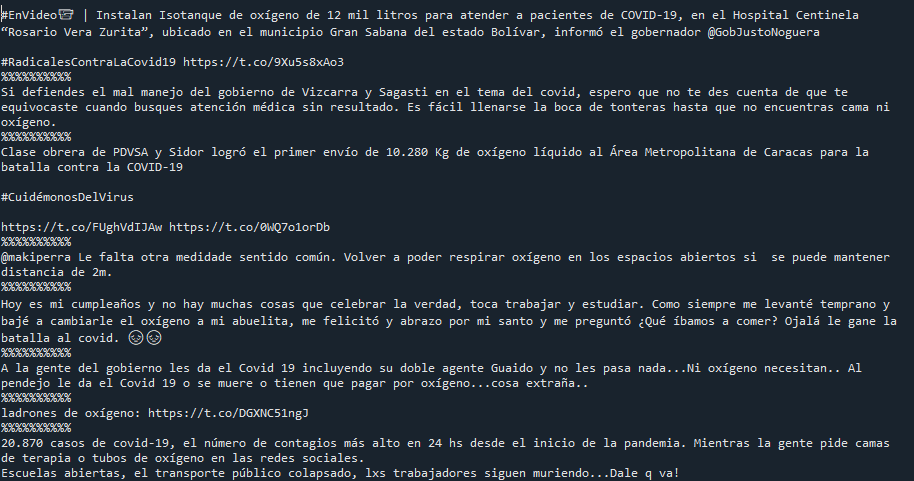
\includegraphics[width=0.95\linewidth]{img/tweets_raw}
	\caption{Imagen que muestra algunas de las publicaciones en bruto sobre la palabra ``oxígeno''. Se muestra en imagen porque algunos caracteres no son manejables en \LaTeX.}
	\label{fig:tweets_raw}
\end{figure}

\paragraph{Separación.} La separación consiste en en segmentar el texto completo en una lista de elementos donde cada elemento sea una publicación, luego separar las en palabras tentativas cada publicación. A continuación se muestran los \textit{tweets} de la Fig~\ref{fig:tweets_raw} después de la separación donde se resaltan los términos problemáticas en rojo\footnote{Pudiera parecer sorprendente que términos como \textit{psvsa} hayan sido reconocidos, pero en efecto forman parte del CREA.}; mientras que en azul se resultan los términos poco frecuentes:

\begin{quote}
	\textcolor{red}{}Instalan \textcolor{red}{Isotanque} de oxígeno de \textcolor{red}{12} mil litros para atender a pacientes de \textcolor{red}{COVID} \textcolor{red}{19} en el Hospital Centinela Rosario Vera Zurita ubicado en el municipio Gran Sabana del estado Bolívar informó el gobernador \textcolor{red}{@GobJustoNoguera} \textcolor{red}{\#RadicalesContraLaCovid19} \textcolor{red}{} 
	\vspace{12pt} \\
	\textcolor{red}{}Si defiendes el mal manejo del gobierno de \textcolor{blue}{Vizcarra} y Sagasti en el tema del \textcolor{red}{covid} espero que no te des cuenta de que te equivocaste cuando busques atención médica sin resultado Es fácil llenarse la boca de \textcolor{blue}{tonteras} hasta que no encuentras cama ni oxígeno \textcolor{red}{} 
	\vspace{12pt} \\
	\textcolor{red}{}Clase obrera de PDVSA y Sidor logró el primer envío de \textcolor{red}{10} \textcolor{red}{280} Kg de oxígeno líquido al Área Metropolitana de Caracas para la batalla contra la \textcolor{red}{COVID} \textcolor{red}{19} \textcolor{red}{\#CuidémonosDelVirus} \textcolor{red}{} 
	\vspace{12pt} \\
	\textcolor{red}{}\textcolor{red}{@makiperra} Le falta otra \textcolor{red}{medidade} sentido común Volver a poder respirar oxígeno en los espacios abiertos si se puede mantener distancia de \textcolor{red}{2m} \textcolor{red}{} 
	\vspace{12pt} \\
	\textcolor{red}{}Hoy es mi cumpleaños y no hay muchas cosas que celebrar la verdad toca trabajar y estudiar Como siempre me levanté temprano y bajé a cambiarle el oxígeno a mi abuelita me felicitó y abrazo por mi santo y me preguntó Qué íbamos a comer Ojalá le gane la batalla al \textcolor{red}{covid} \textcolor{red}{} 
	\vspace{12pt} \\
	\textcolor{red}{}A la gente del gobierno les da el \textcolor{red}{Covid} \textcolor{red}{19} incluyendo su doble agente \textcolor{red}{Guaido} y no les pasa nada Ni oxígeno necesitan Al pendejo le da el \textcolor{red}{Covid} \textcolor{red}{19} o se muere o tienen que pagar por oxígeno cosa extraña \textcolor{red}{} 
	\vspace{12pt} \\
	\textcolor{red}{}ladrones de oxígeno \textcolor{red}{} 
	\vspace{12pt} \\
	\textcolor{red}{}\textcolor{red}{20} \textcolor{red}{870} casos de \textcolor{red}{covid} \textcolor{red}{19} el número de contagios más alto en \textcolor{red}{24} hs desde el inicio de la pandemia Mientras la gente pide camas de terapia o tubos de oxígeno en las redes sociales Escuelas abiertas el transporte público colapsado \textcolor{red}{lxs} trabajadores siguen muriendo Dale q va \textcolor{red}{} 
	\vspace{12pt} \\
	\textcolor{red}{} \textcolor{red}{@canarias7} Sanidad los expertos que no existen y la madre que los parió a todos El oxígeno gratuito y es de todos quienes se creen dueños para permitir si respiramos o no en nuestro descanso y más en la playa o el campo \textcolor{red}{} 
	\vspace{12pt} \\
	\textcolor{red}{}\textcolor{red}{@abc} es Desobediencia civil y no hacer caso de un gobierno corrupto con conflicto de intereses en la venta de mascarillas No al bozal mi vida mi oxígeno Prohibición de mascarilla al aire libre ya \textcolor{red}{} 
\end{quote}

\paragraph{Segmentación.} La segmentación emplea los algoritmos descritos en la sección~\ref{sec:sec33}. La aplicación lleva a obtener lo siguiente:

\begin{quote}
	Instalan \textcolor{red}{Isotanque} de oxígeno de \textcolor{red}{12} mil litros para atender a pacientes de \textcolor{red}{COVID19} en el Hospital Centinela Rosario Vera Zurita ubicado en el municipio Gran Sabana del estado Bolívar informó el gobernador \textcolor{red}{@GobJustoNoguera} radicales contra la \textcolor{red}{covid19} 
	\vspace{12pt} \\
	Si defiendes el mal manejo del gobierno de \textcolor{blue}{Vizcarra} y Sagasti en el tema del \textcolor{red}{covid} espero que no te des cuenta de que te equivocaste cuando busques atención médica sin resultado Es fácil llenarse la boca de \textcolor{blue}{tonteras} hasta que no encuentras cama ni oxígeno 
	\vspace{12pt} \\
	Clase obrera de PDVSA y Sidor logró el primer envío de \textcolor{red}{10280} Kg de oxígeno líquido al Área Metropolitana de Caracas para la batalla contra la \textcolor{red}{COVID19} \textcolor{blue}{cuidémonos} del virus 
	\vspace{12pt} \\
	\textcolor{red}{@makiperra} Le falta otra \textcolor{red}{medidade} sentido común Volver a poder respirar oxígeno en los espacios abiertos si se puede mantener distancia de \textcolor{red}{2m} 
	\vspace{12pt} \\
	Hoy es mi cumpleaños y no hay muchas cosas que celebrar la verdad toca trabajar y estudiar Como siempre me levanté temprano y bajé a cambiarle el oxígeno a mi abuelita me felicitó y abrazo por mi santo y me preguntó Qué íbamos a comer Ojalá le gane la batalla al \textcolor{red}{covid} 
	\vspace{12pt} \\
	A la gente del gobierno les da el \textcolor{red}{Covid19} incluyendo su doble agente \textcolor{red}{Guaido} y no les pasa nada Ni oxígeno necesitan Al pendejo le da el \textcolor{red}{Covid19} o se muere o tienen que pagar por oxígeno cosa extraña 
	\vspace{12pt} \\
	ladrones de oxígeno 
	\vspace{12pt} \\
	\textcolor{red}{20870} casos de \textcolor{red}{covid19} el número de contagios más alto en \textcolor{red}{24} hs desde el inicio de la pandemia Mientras la gente pide camas de terapia o tubos de oxígeno en las redes sociales Escuelas abiertas el transporte público colapsado \textcolor{red}{lxs} trabajadores siguen muriendo Dale q va 
	\vspace{12pt} \\
	\textcolor{red}{@canarias7} Sanidad los expertos que no existen y la madre que los parió a todos El oxígeno gratuito y es de todos quienes se creen dueños para permitir si respiramos o no en nuestro descanso y más en la playa o el campo 
	\vspace{12pt} \\
	\textcolor{red}{@abc} es Desobediencia civil y no hacer caso de un gobierno corrupto con conflicto de intereses en la venta de mascarillas No al bozal mi vida mi oxígeno Prohibición de mascarilla al aire libre ya 
\end{quote}

\paragraph{PoS y NER.} Las tareas de PoS y NER fueron realizadas usando el Stanford CoreNLP \textit{v4.2}. Los modelos desarrollados por la Universidad de Stanford pueden usarse para realizar un pre-procesamiento completo en inglés y ofrece soporte parcial de algunas tareas para Árabe, Chino, Fránces, Alemán y Español \citep{manning2014stanford}.

\paragraph{Lematizado.}

\section{Estimación del modelo}











\chapter{Resultados}
\label{ch:chap4}

En esta sección se presentan varios resultados y la mayoría pueden explorarse de manera casi independiente uno de otro. Sin embargo, todos los resultados presentados en la tesis, salvo los resultados presentados en la sección~\ref{sec:sec41}, están reducidos a las 40,000 palabras de uso más frecuente con base en el CREA.

\section{Corpus}
\label{sec:sec41}

\section{Análisis de las proyecciones}
El \textit{embedding} de palabras es la representación de $N$ palabras en un subespacio de $\mathbb{R}^K$ de dimensión entre 100 y 600. Bajo la métrica coseno, por ejemplo, la palabra \textit{madre} está altamente relacionada\footnote{En este ejemplo, se empleó un corte arbitrario de 0.75 para determinar esto. En la literatura no autor que especifique donde se debe hacer el corte para recuperar las palabras ``similares''.} con la palabras: \textit{padre}, \textit{hija}, \textit{mamá}, \textit{hermana} y \textit{abuela}. 

El ejemplo es un excelente ejemplo de como la métrica coseno recupera relacionadas. Pero es necesario hacer notar que la métrica no establece una relación de orden adecuada. Mayor cercanía debería traducirse en mayor parecido en significado. Pero, en el ejemplo mencionado se tiene que la distancia de \textit{madre} con \textit{padre} fue de 0.76, de \textit{madre} con \textit{hija} fue de 0.81, de \textit{madre} con \textit{mamá} fue de 0.78, de \textit{madre} con \textit{hermana} fue de 0.77 y, de \textit{madre} con \textit{abuela} de 0.75. Por lo tanto, la palabra \textit{hija} está más relacionada con la palabra \textit{madre} \textit{madre} que la palabra \textit{mamá}.

Otro detalle particular radica en determinar un criterio para determinar ``alta'' similaridad. Al relajar el criterio de similaridad la palabra \textit{madre} se encuentra relacionada con varias palabras como \textit{mujer}, \textit{familia}, \textit{marido}, \textit{nuera}, \textit{tía}. Palabras que con claridad tienen una relación con la palabra \textit{madre}. Esto permite establecer un campo semántico donde existen todo tipo de relaciones: Meronomia, donde por ejemplo, \textit{madre} e \textit{hija} forman parte de \textit{familia}; Sinonimia en la relación de \textit{madre} con \textit{mamá}; Hiponimia en la relación \textit{abuela} y \textit{madre} y; Lineales en la relación \textit{madre} e \textit{hija}.

Sin embargo, bajo ese mismo umbral de similaridad, la palabra \textit{vida} resulta similar a \textit{cotidiana}. Lo cual da sentido pues ``vida cotidiana'' es un compuesto común; pero no rescata la misma información que se rescata de la palabra \textit{madre} pues \textit{cotidiana} no forma parte del campo semántico de \textit{vida} por si misma; aunque \textit{vida cotidiana} sí podría considerarse parte del campo semántico de \textit{vida}\footnote{Los ejemplos mencionados son producto de un análisis exhaustivo de la información contenida \texttt{distance\_angle.np} y requiere al menos 13 GB de RAM dispoible para su carga completa.}.

Entonces que significan las p

\section{Propuestas en pre-procesamiento del español}


\section{Análisis de métricas}

La metodología descrita en el capítulo~\ref{ch:chap3} permite obtener 

\section{Aplicaciones}

Dentro del PLN existen tareas que podrían llamarse nucleares como lo es la modelación del lenguaje, el cual es el tema principal de este trabajo, y tareas que podrían llamarse como finales o aplicaciones que son la parte visible del PLN. De acuerdo con \cite{srinivasa2018natural} dentro de estas aplicaciones están los asistentes virtuales, las herramientas de atención al cliente como los chatbots, el análisis de sentimiento y la clasificación de documentos. En esta última parte de los resultados se presentan algunas aplicaciones desarrolladas soportadas en parte de los resultados obtenidos previamente mencionados: Bot Agricultor, Analizador de Opiniones de Foros Educativos y Facebook Miner\footnote{Cada una de las aplicaciones surgió de las pláticas con otras personas que me contaron una idea y que en su momento me pareció una buena para poner a prueba parte de los resultados obtenidos en este trabajo.}. 

\subsection{Bot Agricultor}

A través del Sistema Nacional del Información e Integración de Mercados (SNIIM) la Secretaría de Economía proporciona información histórica sobre tres mercados importantes en el país: agrícola, pecuario y pesquero. En 2018 Detags y la Universidad Autónoma de Querétaro acercaron la información del mercado agrícola al pequeño y mediano agricultor con un resultado favorable por medio de una plataforma de Shiny R y de la experiencia obtenida surgieron dos peticiones: precios futuros y consultas sencillas e informativas \citep{detags}. El bot agricultor representa una solución a la petición de consultas sencillas\footnote{A diferencia de código fuente usado a lo largo de este trabajo, el Bot Agricultor se encuentra en el siguiente repositorio: \url{https://github.com/Wilfridovich17/germinando}.}.

El bot agricultor es un chatbot. Un chatbot, de acuerdo con \cite{khan2017build} es un programa que procesa lenguaje natural del usuario y genera una respuesta útil al usuario; aunque en la práctica la mayoría sigue una estructura basada en reglas donde se le va pidiendo al usuario que responda una pregunta con alguna de las opciones válidas mostradas en pantalla para al final dar respuesta a la solicitud (Fig~\ref{fig:chatbots}).

\begin{figure}[h]
	\centering
	\begin{subfigure}{0.45\linewidth}
		\centering
		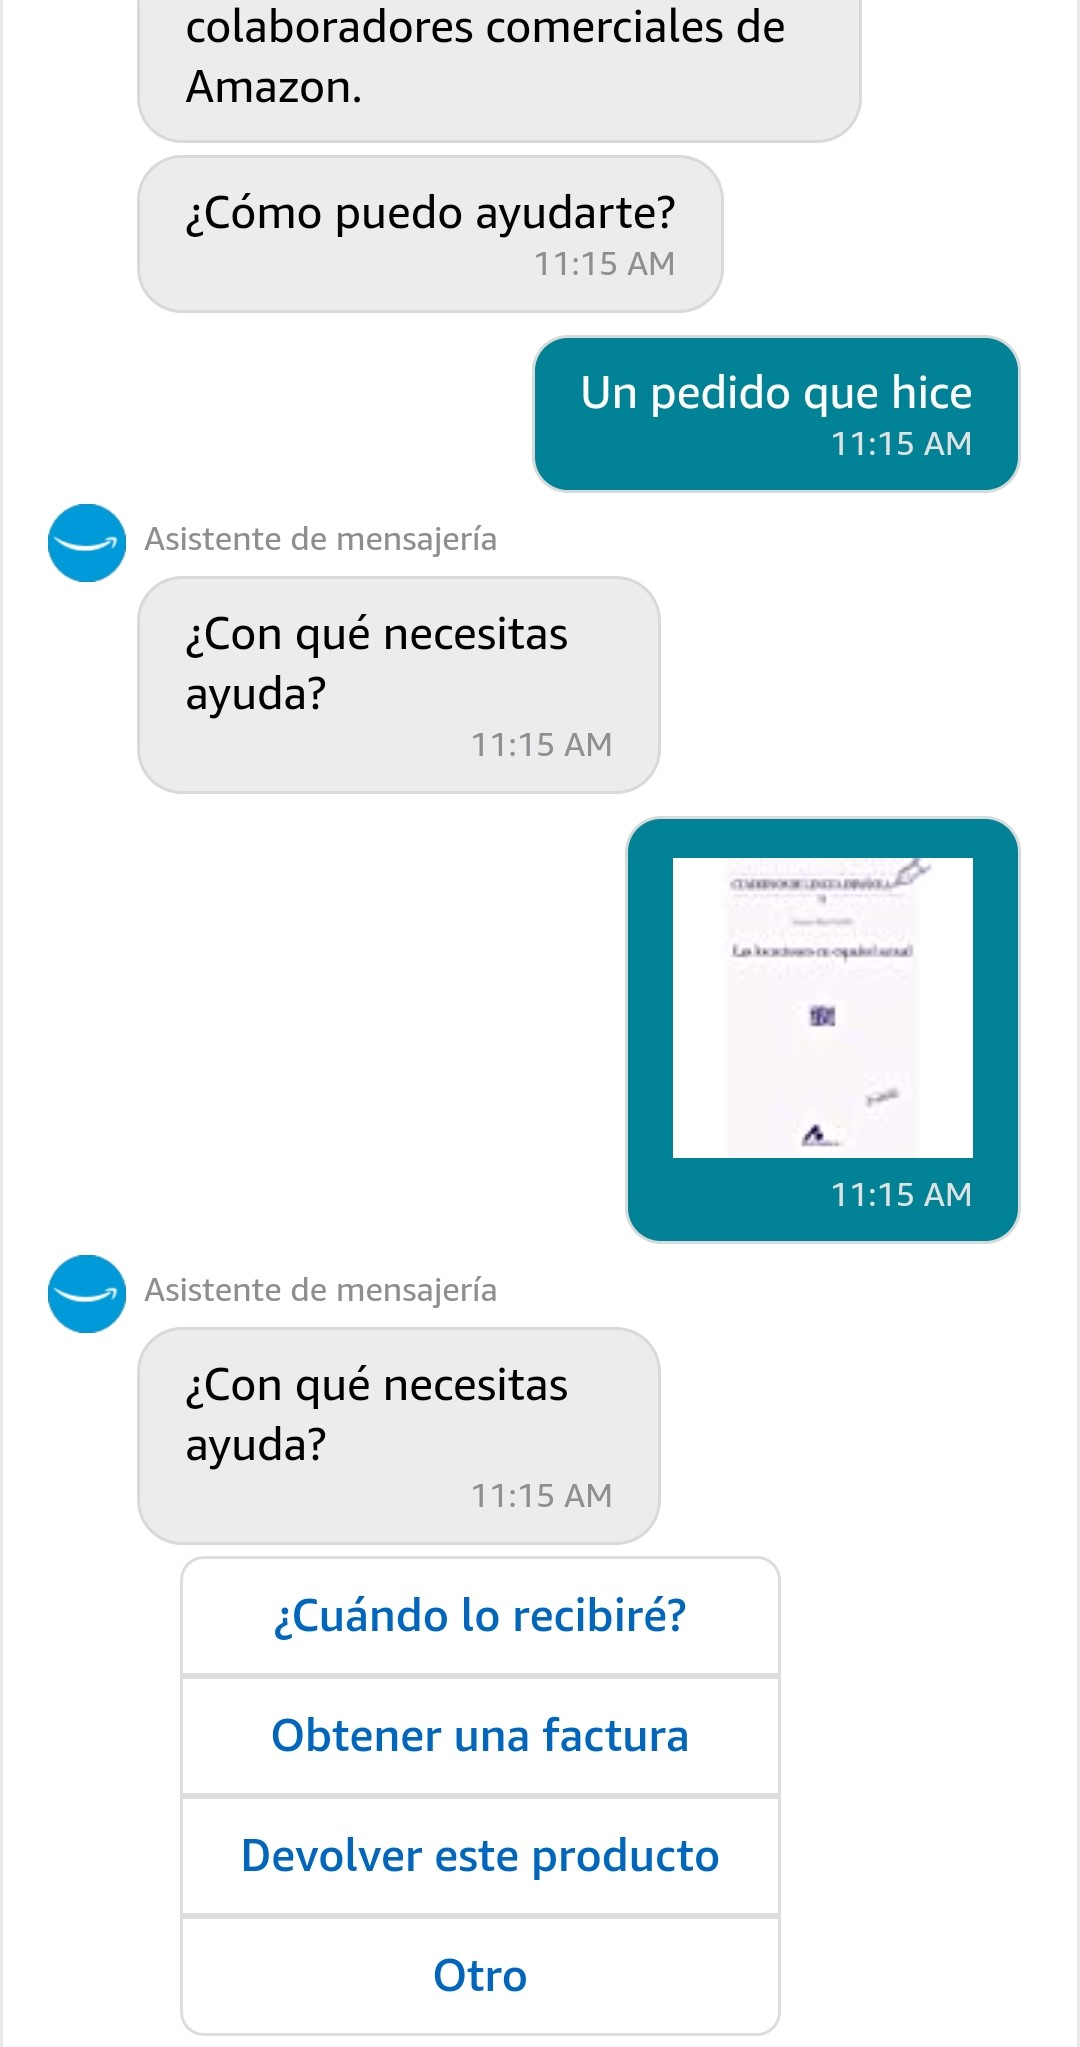
\includegraphics[width=0.45\linewidth]{img/chatbotamazon2}
		\caption{Chatbot de Amazon}
		\label{fig:chatbotamazon}
	\end{subfigure}
	\begin{subfigure}{0.45\linewidth}
		\centering
		
\includegraphics[width=0.45\linewidth]{img/chabotscihub}
		\caption{Chatbot del Sci-Hub}
		\label{fig:chatbotscihub}
	\end{subfigure}
	\begin{subfigure}{0.45\linewidth}
		\centering
		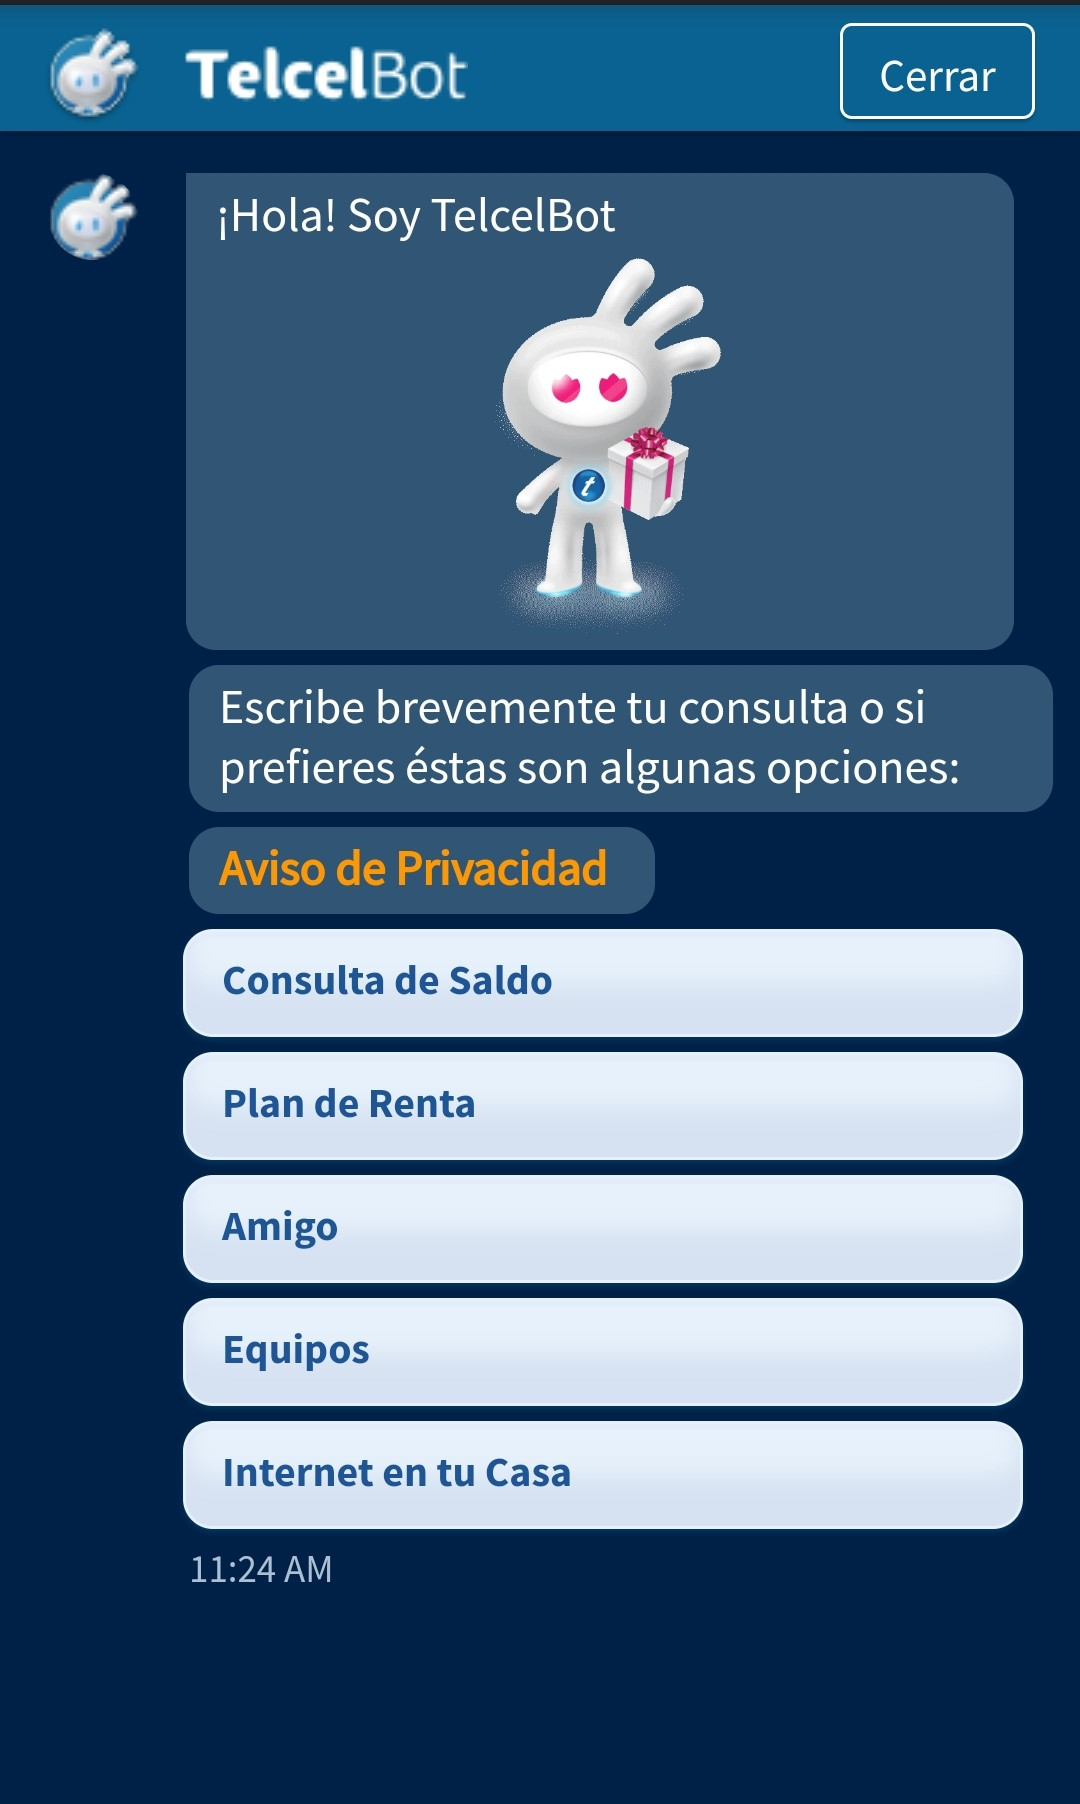
\includegraphics[width=0.45\linewidth]{img/chatbottelcel}
		\caption{Chatbot de Telcel}
		\label{fig:chatbottelcel}
	\end{subfigure}
	\begin{subfigure}{0.45\linewidth}
		\centering
		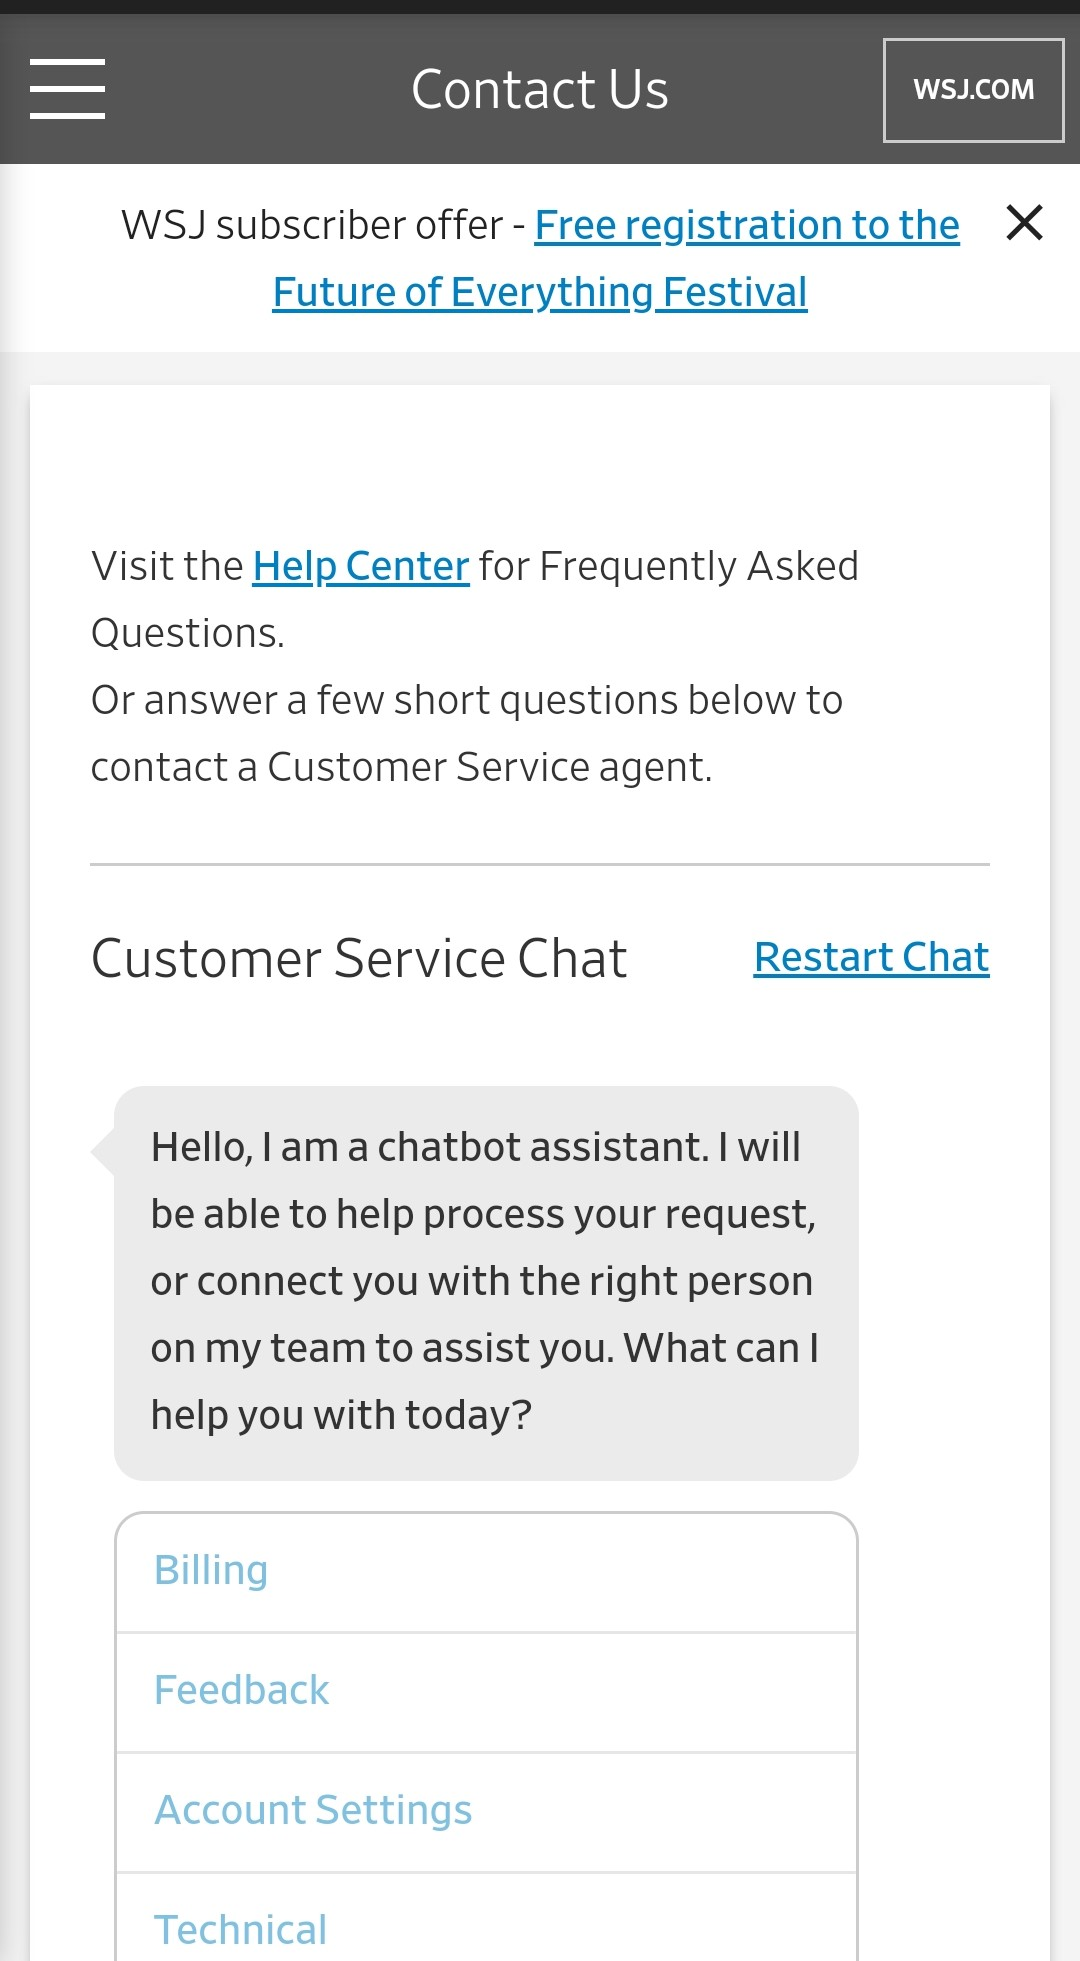
\includegraphics[width=0.45\linewidth]{img/chatbotwsj}
		\caption{Chatbot del Wall Street Journal}
		\label{fig:chatbotwsj}
	\end{subfigure}
	\caption{Ejemplos de chatbots. Obtenidos mediante una captura del pantalla al sitio del proveedor del servicio al interactuar con el chatbot.}
	\label{fig:chatbots}
\end{figure}

En el contexto de las consultas al SNIIM se definieron cuatro tipos de peticiones que fueron clasificadas en: resumen, predicción, precios (históricos) y comparación, las cuales se implementaron en un chatbot de Telegram similar al empleado por Sci-Hub\footnote{Para más información para la creación de un bot en Telegram se puede consultar la siguiente liga \url{https://core.telegram.org/bots}}. Tales peticiones tienen una estructura básica de solicitud:

\begin{itemize}
	\item \texttt{@Resumen Aguacate Hass en Querétaro}
	\item \texttt{@Precio Aguacate Hass en Queretaro 17-04-2020}             
	\item \texttt{@Predice Aguacate Hass en Queretaro 7 días}            
	\item \texttt{@Compara Aguacate Hass en Queretaro 40}
\end{itemize}

Estas instrucciones se traducen de manera sencilla a una \textit{orden} la cual se maneja usando un diccionario de Python. Por ejemplo la instrucción \textit{predice} se codifica como sigue:

\begin{center}
	\texttt{orden = \textbraceleft`instruccion':`resumen', `producto':[[`Aguacate Hass']], `mercado':[[28]], `auxiliares':\textbraceleft`Ventana':7, `Longitud':1\textbraceright\textbraceright}
\end{center}

Las solicitudes con estructura básica fueron creadas para que quien interactúe con el chatbot conozca de antemano qué está pidiendo y qué va a terminar entendiendo el chatbot. Sin embargo, se agregó al chatbot un módulo de lenguaje natural, módulo que le permite transformar instrucciones \textit{más naturales} en la estructura de orden antes mencionada (Fig.~\ref{fig:natbot1}). Mientras que, a nivel usuario, las solicitudes son procesadas como se muestra en la Fig.~\ref{fig:natbot2}.

\begin{figure}[h]
	\centering
	\begin{subfigure}{0.45\linewidth}
		\centering
		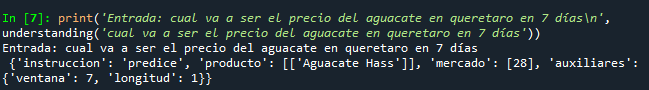
\includegraphics[width=0.9\linewidth]{img/naturalbot1}
		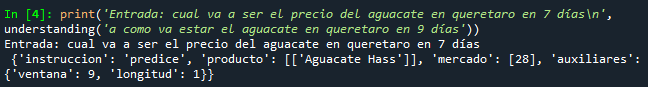
\includegraphics[width=0.9\linewidth]{img/naturalbot2}
		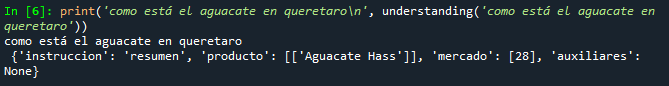
\includegraphics[width=0.9\linewidth]{img/naturalbot3}
		\caption{Ejemplo del funcionamiento del módulo de procesamiento natural del bot agricultor.}
		\label{fig:natbot1}
	\end{subfigure}
	\begin{subfigure}{0.45\linewidth}
		\centering
		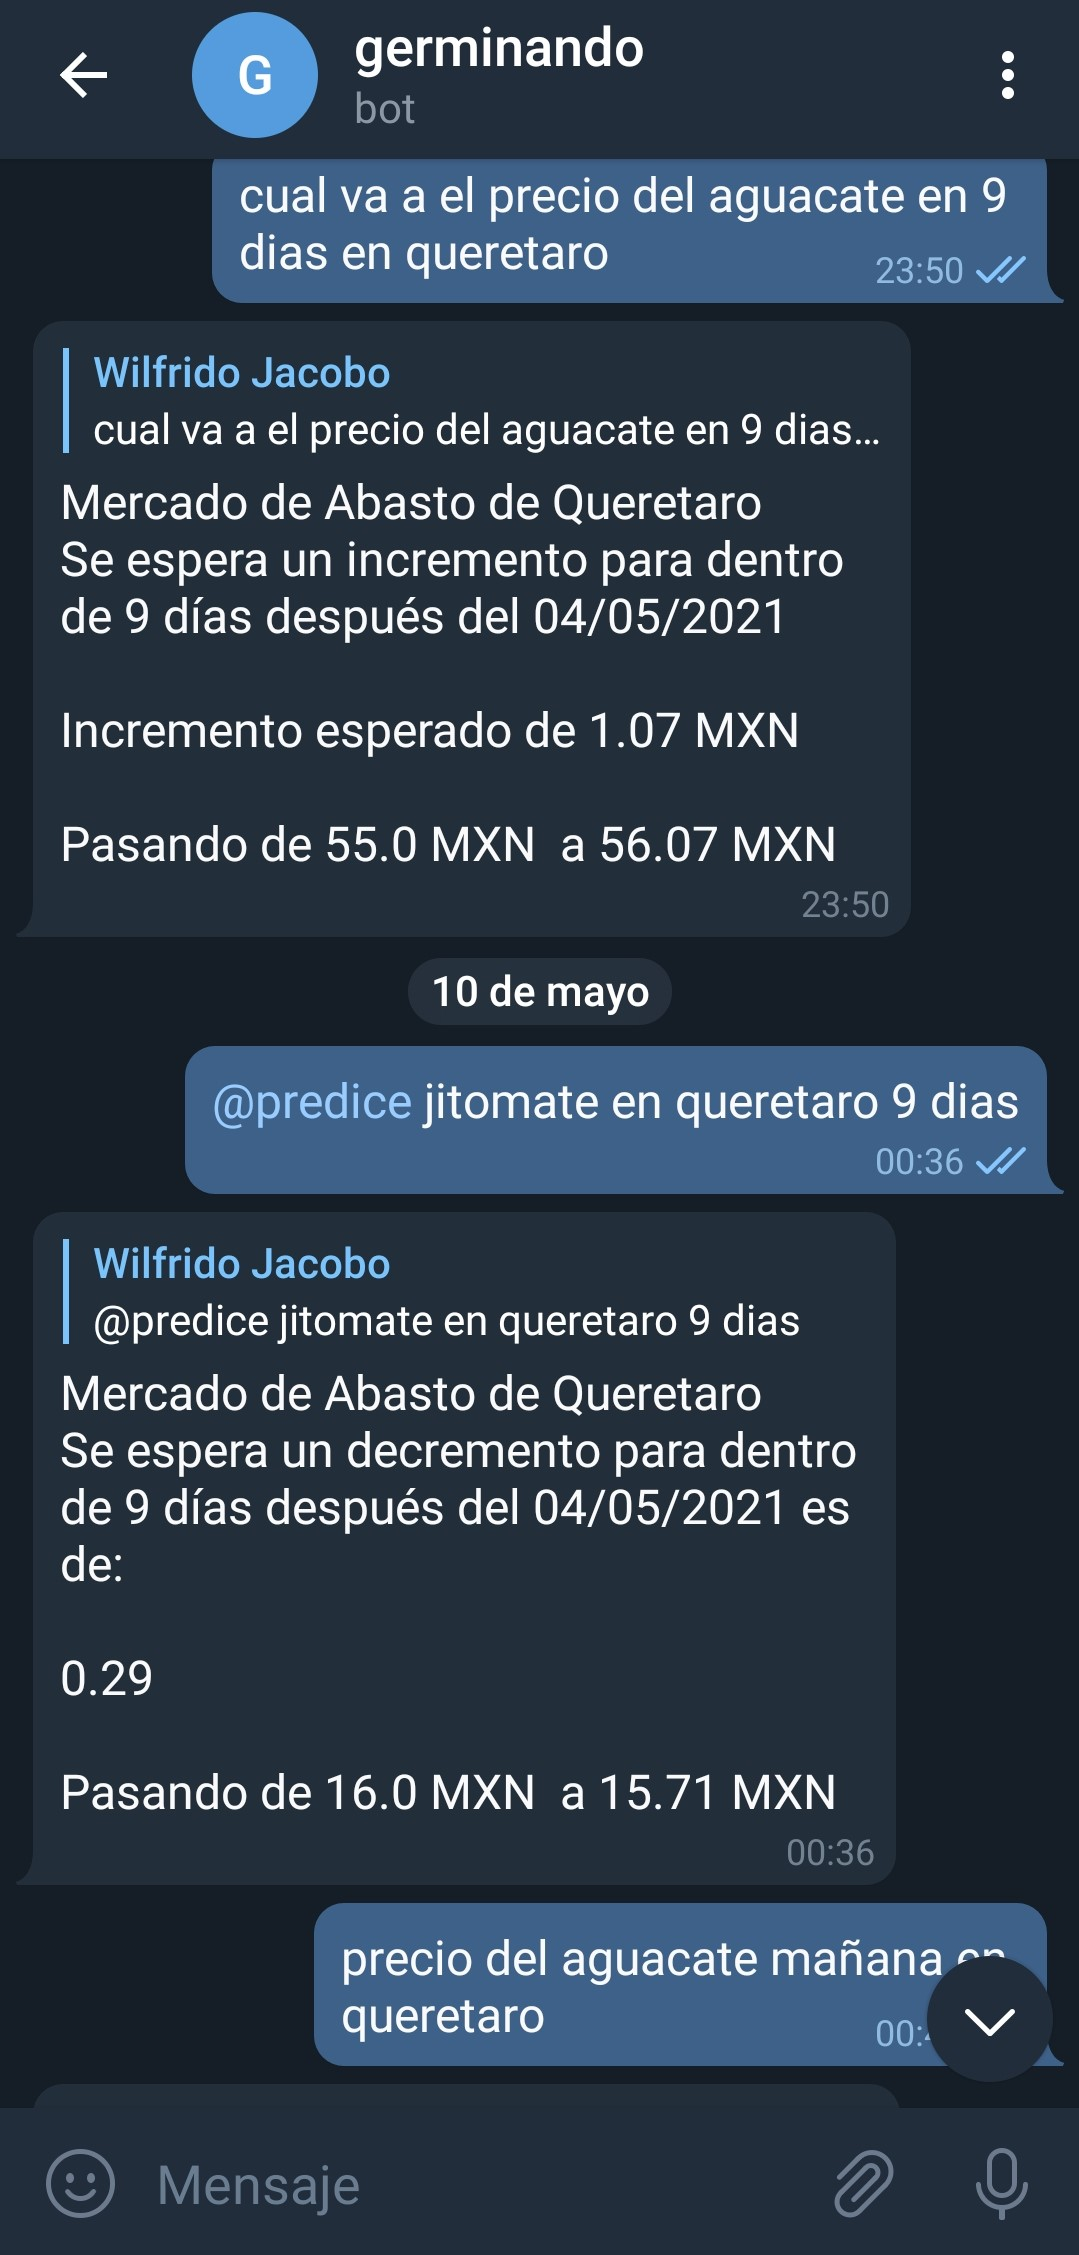
\includegraphics[width=0.45\linewidth]{img/germinandobot}
		\caption{Ejemplo del funcionamiento del bot agricultor a nivel usuario.}
		\label{fig:natbot2}
	\end{subfigure}
	\caption{Bot agricultor donde se muestra la parte trasera del desarrollo y la parte frontal del desarrollo. }
	\label{fig:naturalbot}
\end{figure}


\subsection{Facebook Miner}



\subsection{Análisis de opinión en foros educativos}

De acuerdo con \cite{coviddocentes} para el Banco de Desarrollo Inter-Americano, en la educación a distancia ocasionada por la crisis provocada por el SARS-CoV-2, los profesores sienten que deben estar 24/7 para sus alumnos y dicen sentirse abrumados debido a que reciben una enorme cantidad de llamadas y mensajes fuera de su horario laboral. Además, \cite{teachingcovid} mencionan que la carga laboral de los docentes aumentó drásticamente debido a la generación y adecuación del material para su distribución vía web así como el registro completo de todas las actividades. Sin embargo, el incremento de la carga docente es resultado de las medidas para disminuir la deserción escolar al mantener actividades y contacto con los estudiantes en un horario extendido.

Algunas escuelas dentro de sus medidas para mantener la interacción, han optado por crear foros de discusión para las materias de los estudiantes y fomentar la reflexión e intercambio de ideas entre los estudiantes. Sin embargo, a diferencia del aula tradicional donde la retroalimentación y moderación del docente se realizaba al momento, disponibilidad de los foros impide que los docentes intervengan de manera fluida. En ese sentido, el PLN puede ofrecer una solución parcial mediante una adecuación de un análisis de opinión semántico con el fin de corregir el rumbo de estudiantes que han llegado a una idea que pueda clasificarse de alguna manera como contradictoria.





 


\chapter{Conclusiones}



\appendix

\chapter{Diccionario de términos lingüisticos}






\bibliographystyle{apalike-es}
\bibliography{referencias.bib}


\end{document}